 \chapter[The 23$^{\text{d}}$ of May 2024 - Proper residual \& strategy]{Proper residual \& strategy}

\begin{chapabstract}
	Meeting report
\end{chapabstract}


\minitoc

\section{Proper residual}
\subsection{Idea}
When assessing the loss residual on the continuous interpolated solution, the discretisation error pollutes the loss term. It can thus be interesting to remove its contribution to the loss by restricting the test functions to functions living in the space spanned by the shape functions used for the FE interpolation.

The objective is therefore to minimise the residual
\begin{equation}
	\mathcal{R} = - \int_{\Omega} \eps\left(\vect{u}\right):\ftensor{K}:\eps\left(\vect{u^*}\right) \d \Omega + \int_{\Omega} \vect{f}\cdot \vect{u^*}\d \Omega, \forall \vect{u^*} \in \left( \text{Span}\left(\left\{N_i\left(\vect{x}\right)\right\}_{i\in \llbracket 1,n \rrbracket}\right) \cap \mathcal{H}_0^1\left(\Omega\right)\right)
\end{equation}

\subsection{Results}

To achieve such a goal the loss has been implemented as the sum of all squared residuals associated to each shape function
\begin{equation}
	\mathcal{L} = \sum_{i = 1}^{N}  \left( \mathcal{R}_i \right)^2, 
\end{equation}
with $\mathcal{R}_i =  - \int_{\Omega} \eps\left(\vect{u}\right):\ftensor{K}: N_i\left(\vect{x}\right) \d \Omega + \int_{\Omega} \vect{f}\cdot N_i\left(\vect{x}\right)\d \Omega$.

The convergence process goes to low values of the loss but requires a high number of iterations using the standard ADAM as shown in \cref{fig:ConvergenceResidual_2D}.

\begin{figure}
	\begin{subfigure}[t]{0.5\linewidth}
	\centering
	\includegraphics[width=\linewidth]{Figures/Loss_residual_ADAM_square.pdf}
	\caption{Loss decrease - Adam, $N = 138$}
	\end{subfigure}
	\begin{subfigure}[t]{0.5\linewidth}
		\centering
		\includegraphics[width=\linewidth]{Figures/Loss_residual_ADAM_square_finerMesh.pdf}
	\caption{Loss decrease - Adam, $N = 366$}
	\end{subfigure}  
		\begin{subfigure}[t]{0.5\linewidth}
		\centering
		\includegraphics[width=\linewidth]{Figures/Loss_residual_ADAM_square_MuchfinerMesh.pdf}
		\caption{Loss decrease - Adam, $N = 1166$} 
	\end{subfigure}  
	\caption{Residual loss decrease  for two meshes}
	\label{fig:ConvergenceResidual_2D}
\end{figure}

\begin{figure}
	\begin{subfigure}[t]{0.45\textwidth}
		\captionsetup{skip=-10pt} % local setting for this subfigure
		\centering
		% This file was created with tikzplotlib v0.10.1.
\begin{tikzpicture}[scale=1.0]

\definecolor{darkgray176}{RGB}{176,176,176}
\definecolor{steelblue31119180}{RGB}{31,119,180}

\begin{axis}[
log basis y={10},
tick align=outside,
tick pos=left,
x grid style={darkgray176},
xlabel={Epochs},
xmin=-249.95, xmax=5248.95,
xtick style={color=black},
xtick={-1000,0,1000,2000,3000,4000,5000,6000},
xticklabels={
  $\mathdefault{\ensuremath{-}1000}$,
  $\mathdefault{0}$,
  $\mathdefault{1000}$,
  $\mathdefault{2000}$,
  $\mathdefault{3000}$,
  $\mathdefault{4000}$,
  $\mathdefault{5000}$,
  $\mathdefault{6000}$
},
y grid style={darkgray176},
ylabel={$\mathcal{L}$},
ymin=2.00030357449641e-07, ymax=0.000713270367257533,
ymode=log,
ytick style={color=black},
ytick={1e-08,1e-07,1e-06,1e-05,0.0001,0.001,0.01},
yticklabels={
  $\mathdefault{10^{-8}}$,
  $\mathdefault{10^{-7}}$,
  $\mathdefault{10^{-6}}$,
  $\mathdefault{10^{-5}}$,
  $\mathdefault{10^{-4}}$,
  $\mathdefault{10^{-3}}$,
  $\mathdefault{10^{-2}}$
},
font = \small,
]
\addplot [semithick, steelblue31119180]
table {%
0 0.000491804436466933
1 0.000486021383234991
2 0.000480416265306836
3 0.000474988525886994
4 0.000469735149920439
5 0.000464652852868468
6 0.000459737299171359
7 0.000454983233850982
8 0.00045038523732141
9 0.000445938361179967
10 0.000441638326441909
11 0.000437481287314171
12 0.000433463506047332
13 0.000429581053729379
14 0.00042582968082365
15 0.000422204815761267
16 0.00041870160078714
17 0.000415315019717121
18 0.000412039997233188
19 0.000408871470968431
20 0.000405804453328436
21 0.000402834065182268
22 0.000399955524871167
23 0.00039716416384769
24 0.000394455421015633
25 0.000391824853565227
26 0.000389268126383965
27 0.000386781043014423
28 0.000384359556377327
29 0.000381999793302186
30 0.00037969807577222
31 0.000377450932057785
32 0.000375255122970707
33 0.000373107642609077
34 0.000371005706391158
35 0.000368946763714321
36 0.000366928471424232
37 0.000364948689220056
38 0.00036300546179703
39 0.000361096993655838
40 0.000359221651891586
41 0.000357377940944589
42 0.00035556450091062
43 0.000353780099556144
44 0.000352023605345865
45 0.000350294004854966
46 0.000348590360911143
47 0.000346911818369357
48 0.000345257585458838
49 0.000343626923181428
50 0.000342019125025663
51 0.000340433523444559
52 0.000338869464870374
53 0.000337326331935891
54 0.00033580351623203
55 0.000334300427584047
56 0.00033281650177933
57 0.000331351179657174
58 0.000329903927581959
59 0.000328474220755064
60 0.000327061552125994
61 0.000325665428640756
62 0.000324285364684044
63 0.000322920893231166
64 0.000321571557530535
65 0.000320236909981121
66 0.000318916524012668
67 0.000317609979713631
68 0.000316316879889094
69 0.000315036839583681
70 0.000313769495615569
71 0.000312514498477104
72 0.000311271514965529
73 0.00031004023140428
74 0.000308820347074977
75 0.000307611578487083
76 0.000306413652130572
77 0.000305226306399031
78 0.000304049295363431
79 0.000302882376957238
80 0.000301725324113477
81 0.000300577912920288
82 0.000299439931558207
83 0.000298311178981962
84 0.00029719145616565
85 0.000296080573223799
86 0.000294978345996766
87 0.000293884601405894
88 0.000292799164357312
89 0.00029172187870499
90 0.000290652581648677
91 0.000289591123873332
92 0.000288537358832399
93 0.000287491143645012
94 0.00028645234484456
95 0.000285420830643679
96 0.000284396474089008
97 0.000283379155464326
98 0.000282368756511908
99 0.000281365163952167
100 0.000280368271998871
101 0.000279377975152651
102 0.000278394170490399
103 0.000277416764939952
104 0.000276445661324181
105 0.00027548077029324
106 0.000274522004824665
107 0.000273569280234585
108 0.000272622514404185
109 0.000271681631115082
110 0.000270746548965497
111 0.000269817199449457
112 0.000268893509789251
113 0.000267975412813712
114 0.000267062836586489
115 0.000266155720793691
116 0.000265253998513407
117 0.000264357611575206
118 0.000263466497153275
119 0.000262580597467565
120 0.000261699856531708
121 0.00026082421706492
122 0.000259953628203098
123 0.000259088034526328
124 0.000258227385189744
125 0.000257371628597431
126 0.000256520718050078
127 0.000255674603135232
128 0.000254833240133289
129 0.00025399657933784
130 0.000253164580167721
131 0.000252337194998862
132 0.000251514383568213
133 0.00025069610319299
134 0.000249882313130949
135 0.000249072971505002
136 0.000248268038231891
137 0.000247467477360408
138 0.000246671249305124
139 0.000245879316246602
140 0.000245091642777134
141 0.000244308191162614
142 0.000243528928146447
143 0.000242753817155452
144 0.000241982825148651
145 0.000241215917733579
146 0.000240453060105539
147 0.000239694220502406
148 0.000238939368035892
149 0.000238188469152509
150 0.000237441493579341
151 0.000236698408263017
152 0.000235959188288608
153 0.00023522379942605
154 0.000234492211881533
155 0.000233764395532259
156 0.000233040324643365
157 0.000232319968921164
158 0.000231603299744746
159 0.000230890288570366
160 0.000230180911227119
161 0.000229475137044909
162 0.000228772942044562
163 0.000228074297066917
164 0.000227379176832363
165 0.00022668755731515
166 0.000225999408151997
167 0.000225314707730845
168 0.000224633428294585
169 0.000223955546929184
170 0.000223281038210379
171 0.000222609879031189
172 0.000221942042791783
173 0.000221277506291654
174 0.000220616246012788
175 0.000219958237833928
176 0.000219303457131908
177 0.000218651884605234
178 0.000218003494845397
179 0.000217358263345613
180 0.000216716172333164
181 0.000216077197954323
182 0.000215441318575871
183 0.000214808508548269
184 0.00021417874863986
185 0.000213552018059907
186 0.000212928294450578
187 0.000212307557398121
188 0.000211689782632625
189 0.000211074949915208
190 0.000210463044907534
191 0.000209854042674376
192 0.000209247921258281
193 0.000208644664199725
194 0.000208044249434132
195 0.00020744665458643
196 0.000206851865046686
197 0.000206259857564993
198 0.000205670613709583
199 0.000205084118099266
200 0.000204500347787925
201 0.000203919281408983
202 0.000203340902287733
203 0.000202765197960161
204 0.00020219214320768
205 0.00020162171949668
206 0.000201053910523448
207 0.000200488695847183
208 0.000199926064944541
209 0.000199365992049557
210 0.000198808462324307
211 0.000198253457847864
212 0.000197700965780804
213 0.000197150964161712
214 0.00019660343701685
215 0.000196058367332489
216 0.000195515734271834
217 0.000194975530491003
218 0.000194437733781894
219 0.000193902324522455
220 0.000193369290911703
221 0.000192838613035058
222 0.000192310280578923
223 0.000191784274589673
224 0.000191260576671628
225 0.000190739173404818
226 0.00019022005056602
227 0.000189703192831607
228 0.000189188584739264
229 0.000188676206170865
230 0.000188166044565122
231 0.000187658089848339
232 0.000187152319688321
233 0.000186648723011762
234 0.000186147282866155
235 0.000185647986102636
236 0.000185150820807606
237 0.000184655770020714
238 0.000184162817457086
239 0.000183671955839854
240 0.000183183162466676
241 0.000182696430789994
242 0.00018221174445749
243 0.000181729089030857
244 0.000181248445336065
245 0.000180769808957742
246 0.000180293164358341
247 0.000179818496844052
248 0.000179345792147945
249 0.000178875035266312
250 0.000178406214043275
251 0.000177939319937685
252 0.0001774743382602
253 0.00017701125512083
254 0.000176550055777695
255 0.000176090731972904
256 0.000175633269741402
257 0.000175177654708707
258 0.000174723877160728
259 0.000174271924748085
260 0.000173821783073374
261 0.000173373442282281
262 0.000172926885479167
263 0.000172482108668324
264 0.00017203909557247
265 0.000171597835048799
266 0.000171158312384165
267 0.000170720521428886
268 0.000170284452722634
269 0.000169850088969811
270 0.000169417417941609
271 0.000168986429972969
272 0.000168557118821538
273 0.000168129469506785
274 0.000167703470337134
275 0.000167279109465253
276 0.000166856378250774
277 0.000166435269623855
278 0.000166015766604365
279 0.000165597863973343
280 0.00016518155153018
281 0.000164766810182973
282 0.000164353637261783
283 0.00016394201754622
284 0.000163531944667684
285 0.000163123412804803
286 0.00016271640365916
287 0.00016231091102764
288 0.000161906924647399
289 0.000161504431848367
290 0.000161103427475687
291 0.000160703898959605
292 0.000160305842462578
293 0.000159909242156353
294 0.000159514086974986
295 0.000159120372616308
296 0.000158728091513962
297 0.000158337229750811
298 0.000157947778746924
299 0.000157559729934519
300 0.000157173071016056
301 0.000156787799837875
302 0.000156403907130179
303 0.000156021379243316
304 0.000155640208931913
305 0.000155260387582663
306 0.000154881907053302
307 0.000154504757348154
308 0.00015412893590106
309 0.000153754428787866
310 0.000153381229183032
311 0.000153009324954
312 0.00015263871053667
313 0.000152269381600832
314 0.000151901325493416
315 0.000151534534050074
316 0.000151169001756984
317 0.000150804721152615
318 0.000150441678739326
319 0.000150079874692414
320 0.000149719299638748
321 0.000149359939704487
322 0.000149001794101106
323 0.000148644846738103
324 0.000148289102754195
325 0.000147934543006774
326 0.000147581165737837
327 0.000147228965677871
328 0.00014687792881537
329 0.000146528053300316
330 0.000146179329223139
331 0.000145831750353303
332 0.000145485308583254
333 0.000145140002744902
334 0.000144795818859817
335 0.000144452754592647
336 0.000144110800051286
337 0.000143769946963394
338 0.000143430193495666
339 0.000143091526917962
340 0.000142753947564831
341 0.000142417440722445
342 0.000142082006169123
343 0.000141747635707813
344 0.000141414325191926
345 0.000141082067871774
346 0.000140750854206985
347 0.00014042068002262
348 0.000140091535202094
349 0.000139763416166692
350 0.00013943631764684
351 0.000139110236497759
352 0.000138785161987291
353 0.000138461087907259
354 0.00013813801137698
355 0.000137815925199471
356 0.000137494824868571
357 0.000137174699655813
358 0.000136855548532175
359 0.000136537364758104
360 0.000136220142969852
361 0.000135903874565188
362 0.00013558855696994
363 0.000135274185516075
364 0.000134960753579166
365 0.000134648258324911
366 0.000134336687353925
367 0.000134026040860963
368 0.000133716313182911
369 0.000133407496995759
370 0.000133099587805854
371 0.000132792581919121
372 0.000132486472202385
373 0.000132181256581603
374 0.000131876929723732
375 0.000131573480713972
376 0.00013127090726635
377 0.000130969206718695
378 0.000130668377304069
379 0.000130368406120378
380 0.00013006928742538
381 0.000129771026597872
382 0.000129473615169609
383 0.000129177043063262
384 0.000128881316281526
385 0.000128586418483342
386 0.000128292351896162
387 0.000127999108658661
388 0.000127706688282255
389 0.000127415080294766
390 0.000127124280567433
391 0.000126834291137472
392 0.000126545108013193
393 0.000126256720983602
394 0.00012596912455453
395 0.000125682320897435
396 0.000125396304820717
397 0.000125111065002982
398 0.000124826603973776
399 0.000124542919615955
400 0.000124260000079362
401 0.000123977850154235
402 0.000123696456260683
403 0.00012341582279221
404 0.000123135940840412
405 0.000122856805338194
406 0.000122578414802961
407 0.00012230077150535
408 0.000122023862365493
409 0.000121747685918808
410 0.000121472243193449
411 0.000121197524186041
412 0.000120923526580918
413 0.000120650243623789
414 0.000120377685739583
415 0.000120105838878682
416 0.00011983469742812
417 0.000119564255383933
418 0.000119294519925655
419 0.000119025480455185
420 0.000118757132671215
421 0.000118489475664489
422 0.000118222512405681
423 0.000117956232067938
424 0.000117690629446784
425 0.000117425706851858
426 0.000117161458407691
427 0.000116897878545317
428 0.000116634964564635
429 0.000116372716702389
430 0.000116111135383254
431 0.000115850208253685
432 0.000115589935191304
433 0.000115330316108763
434 0.000115071344723447
435 0.00011481301885625
436 0.000114555331595456
437 0.000114298287738608
438 0.000114041879050259
439 0.000113786101855053
440 0.000113530951718095
441 0.000113276442279081
442 0.000113022555031451
443 0.000112769286914315
444 0.000112516643556741
445 0.000112264612965733
446 0.000112013198002647
447 0.000111762391181566
448 0.00011151219504733
449 0.000111262604624472
450 0.000111013613799498
451 0.000110765223916733
452 0.000110517435860629
453 0.000110270239202443
454 0.000110023633418437
455 0.000109777620575607
456 0.00010953220162208
457 0.000109287364580958
458 0.000109043110315748
459 0.000108799432843369
460 0.000108556335534156
461 0.000108313811288535
462 0.000108071859187067
463 0.000107830476105469
464 0.000107589664474896
465 0.000107349416311953
466 0.000107109728104461
467 0.000106870602778952
468 0.000106632038649398
469 0.000106394026547785
470 0.000106156569156672
471 0.000105919660680946
472 0.000105683306314233
473 0.000105447498562828
474 0.000105212232934728
475 0.000104977517419277
476 0.000104743344634004
477 0.000104509707605696
478 0.000104276605553495
479 0.000104044040682528
480 0.000103812007496373
481 0.000103580502206901
482 0.000103349523506427
483 0.000103119076690971
484 0.000102889150720523
485 0.000102659746422899
486 0.000102430861060264
487 0.000102202495262947
488 0.000101974646246683
489 0.000101747311838237
490 0.000101520486346183
491 0.00010129417475491
492 0.000101068370568318
493 0.000100843069851075
494 0.000100618273044745
495 0.000100393984336167
496 0.000100170195290981
497 9.99469052554342e-05
498 9.97241082536536e-05
499 9.95018119750537e-05
500 9.9280009424085e-05
501 9.90586962294765e-05
502 9.88378730096192e-05
503 9.86175421553378e-05
504 9.83976962397357e-05
505 9.81783351046072e-05
506 9.79594556679043e-05
507 9.7741063344034e-05
508 9.75231499457451e-05
509 9.73057128889984e-05
510 9.70887512785356e-05
511 9.68722692216631e-05
512 9.66562594564387e-05
513 9.64407208432181e-05
514 9.62256516907679e-05
515 9.6011053834055e-05
516 9.57969220380808e-05
517 9.55832548380574e-05
518 9.53700532044552e-05
519 9.51573160730082e-05
520 9.49450397384162e-05
521 9.47332227087954e-05
522 9.45218601392419e-05
523 9.43109573577352e-05
524 9.4100512468216e-05
525 9.3890518448799e-05
526 9.36809737898566e-05
527 9.34718848762555e-05
528 9.32632437500664e-05
529 9.30550498792465e-05
530 9.28473007542398e-05
531 9.26400019137634e-05
532 9.24331455574213e-05
533 9.22267294040778e-05
534 9.2020753305286e-05
535 9.18152193445955e-05
536 9.16101224592113e-05
537 9.14054652412355e-05
538 9.12012429411256e-05
539 9.09974585430272e-05
540 9.07941075739712e-05
541 9.05911836448318e-05
542 9.03886897077842e-05
543 9.01866293156742e-05
544 8.99849960094533e-05
545 8.97837890553218e-05
546 8.95830089404828e-05
547 8.938264974066e-05
548 8.91827183647837e-05
549 8.89832057510471e-05
550 8.8784112927678e-05
551 8.85854396484667e-05
552 8.83871869783244e-05
553 8.81893493462225e-05
554 8.7991929229532e-05
555 8.77949173969792e-05
556 8.75983213057219e-05
557 8.74021384066864e-05
558 8.72063652285847e-05
559 8.70110008947794e-05
560 8.68160502693543e-05
561 8.66215059627583e-05
562 8.64273676776454e-05
563 8.6233636525681e-05
564 8.60403110828713e-05
565 8.58473873886987e-05
566 8.56548645543948e-05
567 8.54627415465897e-05
568 8.52710226657984e-05
569 8.50797022109725e-05
570 8.48887796231809e-05
571 8.46982538882089e-05
572 8.4508127754693e-05
573 8.43183938184775e-05
574 8.41290531087052e-05
575 8.39401050865059e-05
576 8.37515473533633e-05
577 8.35633865250501e-05
578 8.33756087345872e-05
579 8.31882181466685e-05
580 8.30012149297366e-05
581 8.2814600660911e-05
582 8.26283729862239e-05
583 8.24425304469102e-05
584 8.22570697863158e-05
585 8.20719964321223e-05
586 8.18873034779061e-05
587 8.17029891236724e-05
588 8.15190544695915e-05
589 8.13355044605193e-05
590 8.11523332776671e-05
591 8.09695383186233e-05
592 8.07871181529704e-05
593 8.06050758203838e-05
594 8.04234035866948e-05
595 8.02421040392778e-05
596 8.00611753234365e-05
597 7.98806194831878e-05
598 7.97004397654657e-05
599 7.95206286543259e-05
600 7.93411860854527e-05
601 7.91621113405619e-05
602 7.89834054421705e-05
603 7.8805065451413e-05
604 7.86270927049598e-05
605 7.84494834497236e-05
606 7.8272241150934e-05
607 7.80953590687472e-05
608 7.79188387318145e-05
609 7.77426768460211e-05
610 7.75668754247227e-05
611 7.73914411953551e-05
612 7.72163629222436e-05
613 7.70416443528232e-05
614 7.68672807760476e-05
615 7.66932782956231e-05
616 7.65196301917162e-05
617 7.63463369467414e-05
618 7.61733987300949e-05
619 7.6000811815397e-05
620 7.58285780297491e-05
621 7.56566950510704e-05
622 7.54851610600298e-05
623 7.53139826141248e-05
624 7.51431517168442e-05
625 7.4972670977444e-05
626 7.4802540941599e-05
627 7.46327567487558e-05
628 7.44633211963047e-05
629 7.42942266755375e-05
630 7.41254754036744e-05
631 7.39570681628109e-05
632 7.37890097350413e-05
633 7.36212934016543e-05
634 7.34539210102489e-05
635 7.32868888335032e-05
636 7.31201963148643e-05
637 7.29538476719901e-05
638 7.27878336704266e-05
639 7.26221581510566e-05
640 7.24568197293245e-05
641 7.22918222145648e-05
642 7.21271603402446e-05
643 7.19628333858437e-05
644 7.17988423882549e-05
645 7.16351904146205e-05
646 7.14718686145129e-05
647 7.13088781311856e-05
648 7.11462196163615e-05
649 7.09838924024926e-05
650 7.08219004812566e-05
651 7.06602376271314e-05
652 7.0498904973019e-05
653 7.03379042237695e-05
654 7.01772298226148e-05
655 7.00168826442385e-05
656 6.98568610691001e-05
657 6.96971654671297e-05
658 6.95377959643399e-05
659 6.93787550630134e-05
660 6.92200405529569e-05
661 6.90616439483529e-05
662 6.89035714636871e-05
663 6.87458245650104e-05
664 6.85883998051278e-05
665 6.84312955254809e-05
666 6.82745117238549e-05
667 6.81180485998734e-05
668 6.79619045092248e-05
669 6.78060793236844e-05
670 6.76505711095499e-05
671 6.74953795031446e-05
672 6.73405104996263e-05
673 6.71859569305138e-05
674 6.70317199198681e-05
675 6.68777955565411e-05
676 6.67241845088918e-05
677 6.65708906783541e-05
678 6.64179092381139e-05
679 6.62652406605811e-05
680 6.61128855158609e-05
681 6.59608419463007e-05
682 6.58091105857406e-05
683 6.56576881991637e-05
684 6.55065757538258e-05
685 6.53557728163394e-05
686 6.52052819084651e-05
687 6.50550949779764e-05
688 6.49052174708473e-05
689 6.47556478618313e-05
690 6.46063883507414e-05
691 6.44574346007433e-05
692 6.43087824689e-05
693 6.41604356189861e-05
694 6.40123915403286e-05
695 6.3864655277927e-05
696 6.37172197726012e-05
697 6.35700884091435e-05
698 6.34232552272753e-05
699 6.32767274784176e-05
700 6.3130501194568e-05
701 6.29845753068039e-05
702 6.28389492288377e-05
703 6.26936195345276e-05
704 6.25485924762997e-05
705 6.24038638906641e-05
706 6.22594329456336e-05
707 6.21152994426759e-05
708 6.19714594134897e-05
709 6.18279169108497e-05
710 6.16846711110271e-05
711 6.15417205427881e-05
712 6.13990670425757e-05
713 6.12567060145943e-05
714 6.11146384193107e-05
715 6.0972864661074e-05
716 6.08313783509164e-05
717 6.06901884362138e-05
718 6.05492866583771e-05
719 6.04086790788399e-05
720 6.02683670864199e-05
721 6.01283416275948e-05
722 5.99886088692664e-05
723 5.98491600840836e-05
724 5.97100045430229e-05
725 5.95711336172791e-05
726 5.94325452968612e-05
727 5.92942500151663e-05
728 5.91562373119882e-05
729 5.90185079825471e-05
730 5.88810736159489e-05
731 5.87439217229821e-05
732 5.86070569758697e-05
733 5.84704732930668e-05
734 5.83341712202827e-05
735 5.81981534988089e-05
736 5.80624159869798e-05
737 5.79269557819321e-05
738 5.77917827238503e-05
739 5.76568946041241e-05
740 5.75222895269794e-05
741 5.73879624501544e-05
742 5.72539122872311e-05
743 5.71201439455345e-05
744 5.69866524896236e-05
745 5.68534343298615e-05
746 5.67204966646972e-05
747 5.65878340032638e-05
748 5.64554513289204e-05
749 5.63233490312267e-05
750 5.61915204186168e-05
751 5.60599712799855e-05
752 5.59286937156535e-05
753 5.57976868715391e-05
754 5.56669563778464e-05
755 5.55364975914355e-05
756 5.5406314648829e-05
757 5.52764026950063e-05
758 5.51467669333239e-05
759 5.50174060431404e-05
760 5.48883135384896e-05
761 5.47594893529308e-05
762 5.46309388476107e-05
763 5.45026546645556e-05
764 5.43746367184654e-05
765 5.42468923353547e-05
766 5.41194132987406e-05
767 5.39922052860819e-05
768 5.38652684633048e-05
769 5.37385956569351e-05
770 5.36121937654774e-05
771 5.34860558121861e-05
772 5.3360179310239e-05
773 5.32345738082617e-05
774 5.31092297212503e-05
775 5.29841466093149e-05
776 5.28593314273048e-05
777 5.27347772333663e-05
778 5.26104901770744e-05
779 5.24864698136281e-05
780 5.2362708610162e-05
781 5.2239208417793e-05
782 5.21159730055217e-05
783 5.19929950280546e-05
784 5.18702721568344e-05
785 5.17478140070923e-05
786 5.16256126110184e-05
787 5.1503667115012e-05
788 5.13819911484855e-05
789 5.12605730611061e-05
790 5.11394159997517e-05
791 5.10185136879952e-05
792 5.0897865711836e-05
793 5.0777478231292e-05
794 5.06573426456868e-05
795 5.05374603055171e-05
796 5.04178374703081e-05
797 5.02984685714567e-05
798 5.01793583758493e-05
799 5.00605069218874e-05
800 4.99419039409634e-05
801 4.98235521771207e-05
802 4.97054571866057e-05
803 4.95876119074772e-05
804 4.94700171623131e-05
805 4.93526705640415e-05
806 4.92355787986253e-05
807 4.91187356960723e-05
808 4.90021469696018e-05
809 4.88858107876268e-05
810 4.87697216116215e-05
811 4.8653879466635e-05
812 4.85382882958936e-05
813 4.84229445614191e-05
814 4.8307846657425e-05
815 4.81930020078045e-05
816 4.80784014674202e-05
817 4.79640439817725e-05
818 4.78499429361572e-05
819 4.77360849165516e-05
820 4.76224701577629e-05
821 4.7509105997176e-05
822 4.73959826569246e-05
823 4.72831019199884e-05
824 4.71704670956049e-05
825 4.70580737160331e-05
826 4.69459212725969e-05
827 4.68340083365993e-05
828 4.67223479583118e-05
829 4.66109261323727e-05
830 4.64997437205868e-05
831 4.63888065592016e-05
832 4.62781074629317e-05
833 4.61676466874062e-05
834 4.6057428554248e-05
835 4.59474486332854e-05
836 4.58377072656886e-05
837 4.572820718344e-05
838 4.56189513537911e-05
839 4.55099305298134e-05
840 4.54011451942673e-05
841 4.52925998002109e-05
842 4.51842881813427e-05
843 4.5076209735969e-05
844 4.49683716855896e-05
845 4.48607660263297e-05
846 4.47533954928738e-05
847 4.46462572378445e-05
848 4.45393630620696e-05
849 4.44326998360273e-05
850 4.43262687235794e-05
851 4.42200738108276e-05
852 4.41141103648412e-05
853 4.40083759835448e-05
854 4.39028701827885e-05
855 4.37976019854675e-05
856 4.36925622498021e-05
857 4.35877533575571e-05
858 4.34831780653884e-05
859 4.33788375313978e-05
860 4.32747234321359e-05
861 4.31708359327495e-05
862 4.30671817362662e-05
863 4.29637553724398e-05
864 4.28605554210474e-05
865 4.27575866853253e-05
866 4.26548427673545e-05
867 4.25523244866903e-05
868 4.24500303419464e-05
869 4.23479710080974e-05
870 4.2246136616138e-05
871 4.21445248923043e-05
872 4.20431367251315e-05
873 4.19419775056352e-05
874 4.18410404337088e-05
875 4.17403252994204e-05
876 4.16398386880549e-05
877 4.15395725019994e-05
878 4.14395276311588e-05
879 4.13397046221227e-05
880 4.12401141394003e-05
881 4.11407428807322e-05
882 4.10415923572292e-05
883 4.09426603562599e-05
884 4.08439518980148e-05
885 4.07454616751283e-05
886 4.06471902952614e-05
887 4.05491359136889e-05
888 4.04513043385103e-05
889 4.03536909721208e-05
890 4.02562952029671e-05
891 4.01591205060843e-05
892 4.00621667713739e-05
893 3.99654284333209e-05
894 3.98689056036985e-05
895 3.97725975022873e-05
896 3.96765099986786e-05
897 3.95806359544167e-05
898 3.94849780050799e-05
899 3.9389533394359e-05
900 3.92943064275984e-05
901 3.91992920886966e-05
902 3.91044952411651e-05
903 3.90099094044597e-05
904 3.89155420362396e-05
905 3.88213859660135e-05
906 3.87274416072469e-05
907 3.86337074807864e-05
908 3.85401887588497e-05
909 3.84468806947256e-05
910 3.83537818707072e-05
911 3.82608919775917e-05
912 3.81682104289466e-05
913 3.80757482390948e-05
914 3.79834932813078e-05
915 3.78914476146725e-05
916 3.77996101848884e-05
917 3.77079862983493e-05
918 3.76165689632512e-05
919 3.7525358076844e-05
920 3.7434352524737e-05
921 3.7343557754325e-05
922 3.72529696768936e-05
923 3.71625861499238e-05
924 3.7072413730155e-05
925 3.69824449073269e-05
926 3.68926852338761e-05
927 3.68031303483393e-05
928 3.67137783576346e-05
929 3.66246292006181e-05
930 3.65356823761617e-05
931 3.64469428588178e-05
932 3.63584051437035e-05
933 3.62700695935215e-05
934 3.61819351480335e-05
935 3.60940120220984e-05
936 3.60062889889693e-05
937 3.59187662011111e-05
938 3.58314427193732e-05
939 3.57443195557121e-05
940 3.56574007265991e-05
941 3.55706800650181e-05
942 3.54841592245844e-05
943 3.53978360089982e-05
944 3.5311712592615e-05
945 3.5225791352772e-05
946 3.51400723615578e-05
947 3.50545501854499e-05
948 3.49692243043224e-05
949 3.48840944989165e-05
950 3.47991651108582e-05
951 3.47144325094185e-05
952 3.46298950739372e-05
953 3.45455516094614e-05
954 3.44614026759382e-05
955 3.43774473990737e-05
956 3.42936909863776e-05
957 3.42101278395149e-05
958 3.41267639626826e-05
959 3.40435930335296e-05
960 3.39606159861884e-05
961 3.38778357673873e-05
962 3.37952472604961e-05
963 3.37128499529539e-05
964 3.36306424179611e-05
965 3.3548625406688e-05
966 3.34667997647341e-05
967 3.33851692270831e-05
968 3.33037292484853e-05
969 3.3222483670646e-05
970 3.31414289771827e-05
971 3.30605624116929e-05
972 3.29798848930464e-05
973 3.28994002646975e-05
974 3.28191027689679e-05
975 3.27389920296768e-05
976 3.26590677872141e-05
977 3.2579331265641e-05
978 3.2499781243115e-05
979 3.24204235379082e-05
980 3.23412521693611e-05
981 3.22622705644556e-05
982 3.21834734663468e-05
983 3.21048611797518e-05
984 3.20264334157996e-05
985 3.19481950647916e-05
986 3.18701405325953e-05
987 3.17922702425826e-05
988 3.1714583313713e-05
989 3.16370792640178e-05
990 3.15597588543878e-05
991 3.14826207111139e-05
992 3.14056698612289e-05
993 3.13289059706114e-05
994 3.12523216099561e-05
995 3.11759182875793e-05
996 3.10996955949943e-05
997 3.10236533957576e-05
998 3.09477934035128e-05
999 3.08721161197865e-05
1000 3.07966183745166e-05
1001 3.07212997801347e-05
1002 3.06461600106655e-05
1003 3.05711969265565e-05
1004 3.04964130339544e-05
1005 3.04218128828557e-05
1006 3.03473897559876e-05
1007 3.02731503358405e-05
1008 3.01990860859058e-05
1009 3.01251984928283e-05
1010 3.0051488236274e-05
1011 2.99779538756365e-05
1012 2.99045936119062e-05
1013 2.98314095569165e-05
1014 2.97584006365813e-05
1015 2.96855663212009e-05
1016 2.96129110854396e-05
1017 2.9540435282941e-05
1018 2.94681331437098e-05
1019 2.93960028793793e-05
1020 2.93240473913316e-05
1021 2.92522642979084e-05
1022 2.9180652635528e-05
1023 2.91092131828316e-05
1024 2.90379452049582e-05
1025 2.89668550677191e-05
1026 2.88959346308348e-05
1027 2.88251870644593e-05
1028 2.87546101821337e-05
1029 2.86842070177904e-05
1030 2.86139744599858e-05
1031 2.85439117235784e-05
1032 2.84740172675908e-05
1033 2.84042916746283e-05
1034 2.83347358179065e-05
1035 2.82653520137556e-05
1036 2.81961376605865e-05
1037 2.81270918136088e-05
1038 2.80582123827687e-05
1039 2.79895007364284e-05
1040 2.79209563553969e-05
1041 2.78525775775124e-05
1042 2.77843690793784e-05
1043 2.77163266701277e-05
1044 2.76484502323486e-05
1045 2.75807394404646e-05
1046 2.75131933626145e-05
1047 2.74458132732408e-05
1048 2.73786022172287e-05
1049 2.73115545030536e-05
1050 2.72446709108153e-05
1051 2.71779508622135e-05
1052 2.71113942088198e-05
1053 2.70450003105786e-05
1054 2.69787726428493e-05
1055 2.69127079157508e-05
1056 2.68468054334318e-05
1057 2.67810649648518e-05
1058 2.67154846596818e-05
1059 2.66500666000978e-05
1060 2.65848091348823e-05
1061 2.65197123070867e-05
1062 2.64547763869916e-05
1063 2.63899996203419e-05
1064 2.63253834216219e-05
1065 2.62609252658858e-05
1066 2.61966326126861e-05
1067 2.61325017650921e-05
1068 2.60685296862589e-05
1069 2.60047143922262e-05
1070 2.59410575220773e-05
1071 2.58775586604191e-05
1072 2.58142157066033e-05
1073 2.57510309146446e-05
1074 2.5688001640032e-05
1075 2.56251294743084e-05
1076 2.5562413211783e-05
1077 2.54998538644081e-05
1078 2.54374492944881e-05
1079 2.53751998128767e-05
1080 2.53131095150324e-05
1081 2.52511737772804e-05
1082 2.51893916112366e-05
1083 2.51277641414626e-05
1084 2.5066290216067e-05
1085 2.50049681193012e-05
1086 2.49438011283744e-05
1087 2.48827874592165e-05
1088 2.48219263015099e-05
1089 2.47612167086401e-05
1090 2.47006598515171e-05
1091 2.46402539458e-05
1092 2.45799995388621e-05
1093 2.4519899889118e-05
1094 2.44599513268062e-05
1095 2.44001523593628e-05
1096 2.43405038194967e-05
1097 2.42810061421453e-05
1098 2.42216575369579e-05
1099 2.41624595811466e-05
1100 2.41034095154491e-05
1101 2.40445086091814e-05
1102 2.39857561003714e-05
1103 2.39271511206089e-05
1104 2.38686950667706e-05
1105 2.38103855818102e-05
1106 2.37522282733373e-05
1107 2.36942180544545e-05
1108 2.36363539333174e-05
1109 2.3578637235084e-05
1110 2.35210661234541e-05
1111 2.34636425105888e-05
1112 2.34063635459108e-05
1113 2.33492295316273e-05
1114 2.32922413556528e-05
1115 2.32353974321834e-05
1116 2.31786964871339e-05
1117 2.31221411486251e-05
1118 2.30657302374237e-05
1119 2.30094620504164e-05
1120 2.29533386254361e-05
1121 2.28973567276002e-05
1122 2.28415171475952e-05
1123 2.2785821388592e-05
1124 2.2730267498392e-05
1125 2.26748551092417e-05
1126 2.2619585235591e-05
1127 2.25644563438928e-05
1128 2.25094691712243e-05
1129 2.24546232748991e-05
1130 2.23999175030536e-05
1131 2.23453512598506e-05
1132 2.22909258429503e-05
1133 2.22366430728858e-05
1134 2.21824992511621e-05
1135 2.212849503557e-05
1136 2.20746294030482e-05
1137 2.20208997310229e-05
1138 2.19673077089707e-05
1139 2.19138547351434e-05
1140 2.18605399346816e-05
1141 2.18073618589221e-05
1142 2.17543202283771e-05
1143 2.17014165154161e-05
1144 2.16486491480819e-05
1145 2.15960172473091e-05
1146 2.15435221231575e-05
1147 2.14911672529228e-05
1148 2.14389437186224e-05
1149 2.13868552238342e-05
1150 2.13349028517764e-05
1151 2.12830857511644e-05
1152 2.12314027717747e-05
1153 2.11798535254296e-05
1154 2.11284381244349e-05
1155 2.10771561637215e-05
1156 2.10260085530371e-05
1157 2.09749934109593e-05
1158 2.09241067774813e-05
1159 2.08733532605247e-05
1160 2.08227308353901e-05
1161 2.07722458947916e-05
1162 2.07218928062931e-05
1163 2.06716712555217e-05
1164 2.06215816156776e-05
1165 2.05716217226338e-05
1166 2.052178868831e-05
1167 2.0472087105818e-05
1168 2.04225157135015e-05
1169 2.03730747599844e-05
1170 2.03237623902434e-05
1171 2.02745792779597e-05
1172 2.02255262603703e-05
1173 2.01765989186554e-05
1174 2.01277994977699e-05
1175 2.00791285925063e-05
1176 2.0030589650944e-05
1177 1.99821784941236e-05
1178 1.99338942804435e-05
1179 1.98857333054076e-05
1180 1.98376999398618e-05
1181 1.97897932880718e-05
1182 1.97420136968019e-05
1183 1.96943603720558e-05
1184 1.96468327492566e-05
1185 1.95994270751743e-05
1186 1.95521467645528e-05
1187 1.95049923644236e-05
1188 1.94579618950981e-05
1189 1.94110560517852e-05
1190 1.93642783191209e-05
1191 1.93176220102415e-05
1192 1.92710897239414e-05
1193 1.92246805902111e-05
1194 1.91783942584138e-05
1195 1.91322313747114e-05
1196 1.90861873684821e-05
1197 1.9040266131457e-05
1198 1.89944668759125e-05
1199 1.89487892668074e-05
1200 1.89032359131164e-05
1201 1.8857799817629e-05
1202 1.88124850180054e-05
1203 1.87672917010994e-05
1204 1.87222209025109e-05
1205 1.86772742394961e-05
1206 1.86324442417664e-05
1207 1.85877338383832e-05
1208 1.85431435839829e-05
1209 1.84986723016734e-05
1210 1.84543173001371e-05
1211 1.8410079318986e-05
1212 1.8365959674773e-05
1213 1.83219593667642e-05
1214 1.82780736674694e-05
1215 1.82343067421539e-05
1216 1.81906568990045e-05
1217 1.81471241386851e-05
1218 1.81037097962301e-05
1219 1.80604087540923e-05
1220 1.80172281732311e-05
1221 1.79741637662794e-05
1222 1.79312120713656e-05
1223 1.78883784787487e-05
1224 1.78456602981159e-05
1225 1.78030585458987e-05
1226 1.77605681485717e-05
1227 1.77181924212695e-05
1228 1.76759319813702e-05
1229 1.7633785721158e-05
1230 1.75917517881824e-05
1231 1.75498312159213e-05
1232 1.75080241909692e-05
1233 1.74663311759623e-05
1234 1.7424748056646e-05
1235 1.73832816623073e-05
1236 1.73419282760484e-05
1237 1.73006839379466e-05
1238 1.72595521183067e-05
1239 1.72185308537847e-05
1240 1.71776183071173e-05
1241 1.71368172157318e-05
1242 1.70961283747314e-05
1243 1.70555501202069e-05
1244 1.70150793725489e-05
1245 1.69747197733664e-05
1246 1.69344721417127e-05
1247 1.68943325952899e-05
1248 1.6854302828543e-05
1249 1.68143826095368e-05
1250 1.67745688388546e-05
1251 1.67348676872726e-05
1252 1.66952736520272e-05
1253 1.6655785325648e-05
1254 1.66164058999924e-05
1255 1.65771348156828e-05
1256 1.65379685844221e-05
1257 1.64989099138441e-05
1258 1.64599594057802e-05
1259 1.64211138591379e-05
1260 1.63823755185738e-05
1261 1.63437423393864e-05
1262 1.63052130275931e-05
1263 1.62667902385374e-05
1264 1.62284704356281e-05
1265 1.61902571070303e-05
1266 1.61521494653991e-05
1267 1.61141471306363e-05
1268 1.60762502780257e-05
1269 1.60384582012463e-05
1270 1.60007686430445e-05
1271 1.59631834447029e-05
1272 1.59256991343895e-05
1273 1.58883193716624e-05
1274 1.58510438664401e-05
1275 1.58138692407147e-05
1276 1.57767985246013e-05
1277 1.57398289576562e-05
1278 1.57029603417568e-05
1279 1.56661941298353e-05
1280 1.56295273223971e-05
1281 1.55929633339487e-05
1282 1.55564980300701e-05
1283 1.55201369795043e-05
1284 1.54838774804579e-05
1285 1.54477163446508e-05
1286 1.54116568660065e-05
1287 1.53756950621639e-05
1288 1.53398348480339e-05
1289 1.530407359638e-05
1290 1.52684096087337e-05
1291 1.52328463216087e-05
1292 1.51973795321486e-05
1293 1.51620122052459e-05
1294 1.51267416453545e-05
1295 1.50915705107631e-05
1296 1.50564958139378e-05
1297 1.50215197399793e-05
1298 1.49866390019418e-05
1299 1.49518570732009e-05
1300 1.49171745670547e-05
1301 1.488258662662e-05
1302 1.48480972418435e-05
1303 1.48137020465317e-05
1304 1.4779404703774e-05
1305 1.47451996135351e-05
1306 1.47110911611886e-05
1307 1.46770776025913e-05
1308 1.46431600529175e-05
1309 1.46093346745546e-05
1310 1.45756054211594e-05
1311 1.45419695043599e-05
1312 1.45084292013573e-05
1313 1.44749814830301e-05
1314 1.44416269066612e-05
1315 1.44083649101202e-05
1316 1.43751975199948e-05
1317 1.43421242355226e-05
1318 1.43091445613347e-05
1319 1.42762557945419e-05
1320 1.4243462233339e-05
1321 1.4210759779542e-05
1322 1.4178149090757e-05
1323 1.41456285433371e-05
1324 1.41132018113311e-05
1325 1.40808651288919e-05
1326 1.40486170172704e-05
1327 1.40164612344839e-05
1328 1.39843944460861e-05
1329 1.39524200465e-05
1330 1.39205329830107e-05
1331 1.38887373255685e-05
1332 1.3857030458977e-05
1333 1.38254131894181e-05
1334 1.37938868562603e-05
1335 1.37624491017008e-05
1336 1.37311014774082e-05
1337 1.36998399053542e-05
1338 1.36686692299669e-05
1339 1.36375857132138e-05
1340 1.36065903420182e-05
1341 1.35756820821576e-05
1342 1.35448603507724e-05
1343 1.35141273106155e-05
1344 1.34834796490557e-05
1345 1.3452921603497e-05
1346 1.3422449356863e-05
1347 1.33920615252261e-05
1348 1.33617617409238e-05
1349 1.33315471499238e-05
1350 1.33014191685846e-05
1351 1.32713757879179e-05
1352 1.32414196112744e-05
1353 1.32115491807285e-05
1354 1.31817629465145e-05
1355 1.31520605087325e-05
1356 1.31224437180851e-05
1357 1.30929102901249e-05
1358 1.30634598018514e-05
1359 1.30340940351791e-05
1360 1.30048113303653e-05
1361 1.29756117837827e-05
1362 1.29464963412605e-05
1363 1.29174632539315e-05
1364 1.2888512377176e-05
1365 1.28596453141198e-05
1366 1.28308597827577e-05
1367 1.28021560302994e-05
1368 1.27735351428448e-05
1369 1.27449952789653e-05
1370 1.27165391322923e-05
1371 1.26881648445784e-05
1372 1.26598732628257e-05
1373 1.26316606611237e-05
1374 1.26035309797133e-05
1375 1.25754818184145e-05
1376 1.25475112339986e-05
1377 1.25196226893541e-05
1378 1.24918142283926e-05
1379 1.24640836485091e-05
1380 1.24364322215847e-05
1381 1.24088604319169e-05
1382 1.23813683889153e-05
1383 1.23539548355278e-05
1384 1.23266184203048e-05
1385 1.22993625752637e-05
1386 1.22721839695388e-05
1387 1.22450831480588e-05
1388 1.22180601627169e-05
1389 1.21911184191748e-05
1390 1.21642541311448e-05
1391 1.21374655177066e-05
1392 1.21107540853411e-05
1393 1.20841207351353e-05
1394 1.20575638345075e-05
1395 1.20310830802255e-05
1396 1.20046778317446e-05
1397 1.1978350880469e-05
1398 1.195209825119e-05
1399 1.19259227275297e-05
1400 1.18998213930368e-05
1401 1.18737956884427e-05
1402 1.18478472041441e-05
1403 1.18219725958094e-05
1404 1.17961735454686e-05
1405 1.17704476603672e-05
1406 1.17447959664752e-05
1407 1.17192194605077e-05
1408 1.16937198629127e-05
1409 1.16682923272435e-05
1410 1.16429388410854e-05
1411 1.1617657389553e-05
1412 1.15924499659601e-05
1413 1.15673178484796e-05
1414 1.15422572215087e-05
1415 1.15172695608356e-05
1416 1.14923539046757e-05
1417 1.14675109613193e-05
1418 1.14427385358305e-05
1419 1.14180382889188e-05
1420 1.13934115581915e-05
1421 1.1368856667282e-05
1422 1.13443716424328e-05
1423 1.13199579394311e-05
1424 1.12956143841488e-05
1425 1.12713422364127e-05
1426 1.12471395969498e-05
1427 1.12230088175377e-05
1428 1.11989515722993e-05
1429 1.11749651241937e-05
1430 1.11510475987056e-05
1431 1.11272002396813e-05
1432 1.11034215039015e-05
1433 1.10797119701577e-05
1434 1.10560713297114e-05
1435 1.10324999985432e-05
1436 1.10089964332525e-05
1437 1.09855605040248e-05
1438 1.09621938193141e-05
1439 1.0938895111192e-05
1440 1.09156647827958e-05
1441 1.0892501431258e-05
1442 1.08694085781381e-05
1443 1.08463826564985e-05
1444 1.08234246534309e-05
1445 1.08005333406357e-05
1446 1.07777091381259e-05
1447 1.0754951341737e-05
1448 1.07322615194757e-05
1449 1.07096391126751e-05
1450 1.06870824858733e-05
1451 1.06645921611892e-05
1452 1.06421672788536e-05
1453 1.06198087143677e-05
1454 1.05975147038639e-05
1455 1.05752873424693e-05
1456 1.05531257754303e-05
1457 1.05310285627311e-05
1458 1.05089967733735e-05
1459 1.04870293039565e-05
1460 1.04651257481947e-05
1461 1.04432875502894e-05
1462 1.04215126635658e-05
1463 1.03998026535183e-05
1464 1.0378155915214e-05
1465 1.03565721051245e-05
1466 1.03350506144811e-05
1467 1.03135921381113e-05
1468 1.02921975165332e-05
1469 1.02708679152055e-05
1470 1.02496004370484e-05
1471 1.0228396285922e-05
1472 1.0207254129137e-05
1473 1.01861750603929e-05
1474 1.01651577627035e-05
1475 1.01442027261658e-05
1476 1.0123310713397e-05
1477 1.01024796639334e-05
1478 1.00817098004779e-05
1479 1.00610000370382e-05
1480 1.00403511844498e-05
1481 1.00197627160724e-05
1482 9.99923615555713e-06
1483 9.97877008544866e-06
1484 9.95836426638169e-06
1485 9.93802108589054e-06
1486 9.91773755812789e-06
1487 9.8975120006193e-06
1488 9.87734721270305e-06
1489 9.8572417902571e-06
1490 9.83719740398801e-06
1491 9.81721332418865e-06
1492 9.79728865816911e-06
1493 9.77742287579344e-06
1494 9.75761470465223e-06
1495 9.73786532378321e-06
1496 9.71817403169373e-06
1497 9.6985421850467e-06
1498 9.67896814384117e-06
1499 9.65945038708871e-06
1500 9.63999131270011e-06
1501 9.62059007183918e-06
1502 9.6012460063788e-06
1503 9.58196075914082e-06
1504 9.56273088605944e-06
1505 9.54355843506641e-06
1506 9.52444267482265e-06
1507 9.50538504958417e-06
1508 9.48638386867376e-06
1509 9.467436909756e-06
1510 9.44854640664543e-06
1511 9.42971326392204e-06
1512 9.41093814136519e-06
1513 9.39221672021349e-06
1514 9.3735526239169e-06
1515 9.35494521370199e-06
1516 9.33639332573639e-06
1517 9.31789467842842e-06
1518 9.29945204136004e-06
1519 9.28106474162449e-06
1520 9.2627301517485e-06
1521 9.24445045641362e-06
1522 9.22622638010307e-06
1523 9.20805677957861e-06
1524 9.18993964926333e-06
1525 9.17187672568566e-06
1526 9.15386893161808e-06
1527 9.13591304259019e-06
1528 9.11801143364974e-06
1529 9.10016335436356e-06
1530 9.08236681705053e-06
1531 9.06462467678029e-06
1532 9.04693564924913e-06
1533 9.0292980750144e-06
1534 9.01171335465895e-06
1535 8.9941830315958e-06
1536 8.97670466751543e-06
1537 8.95927891543786e-06
1538 8.9419035646135e-06
1539 8.92458073644913e-06
1540 8.9073093676019e-06
1541 8.89008938483263e-06
1542 8.87292111663221e-06
1543 8.85580430357397e-06
1544 8.83873751104644e-06
1545 8.82172208778115e-06
1546 8.80475706043534e-06
1547 8.78784432073503e-06
1548 8.77098231488365e-06
1549 8.75416932204408e-06
1550 8.73740715420393e-06
1551 8.72069377265179e-06
1552 8.70403183262689e-06
1553 8.68741860171968e-06
1554 8.67085583884968e-06
1555 8.65434302605568e-06
1556 8.63787870189359e-06
1557 8.62146399324981e-06
1558 8.60509805933113e-06
1559 8.58878323985427e-06
1560 8.57251635473827e-06
1561 8.5562986160535e-06
1562 8.54012829778236e-06
1563 8.52400704382045e-06
1564 8.50793280331101e-06
1565 8.49190703585265e-06
1566 8.47592931406675e-06
1567 8.46000020651516e-06
1568 8.44411762363181e-06
1569 8.42828325934481e-06
1570 8.41249567557801e-06
1571 8.39675593552996e-06
1572 8.38106222117924e-06
1573 8.36541619066016e-06
1574 8.34981619793108e-06
1575 8.33426448632687e-06
1576 8.3187579969777e-06
1577 8.30329703662464e-06
1578 8.28788335691379e-06
1579 8.27251605082193e-06
1580 8.25719544396354e-06
1581 8.24191984479463e-06
1582 8.2266909442417e-06
1583 8.21150677596265e-06
1584 8.19636889049511e-06
1585 8.18127669445169e-06
1586 8.16622887572347e-06
1587 8.1512281540422e-06
1588 8.13627153665225e-06
1589 8.12135892649791e-06
1590 8.1064918629159e-06
1591 8.09166876570981e-06
1592 8.07689093835015e-06
1593 8.06215627929826e-06
1594 8.04746501433781e-06
1595 8.03281866592869e-06
1596 8.01821586284789e-06
1597 8.00365645244282e-06
1598 7.98914154640825e-06
1599 7.97466944817104e-06
1600 7.96023974199266e-06
1601 7.94585415265814e-06
1602 7.93151145804847e-06
1603 7.91721135386505e-06
1604 7.90295530314329e-06
1605 7.8887410359338e-06
1606 7.8745688258529e-06
1607 7.86044009474068e-06
1608 7.84635360985485e-06
1609 7.83230882827195e-06
1610 7.81830671076302e-06
1611 7.80434752108983e-06
1612 7.79042971767264e-06
1613 7.77655396178405e-06
1614 7.76272094785398e-06
1615 7.74892892144956e-06
1616 7.73517745705623e-06
1617 7.72146696099329e-06
1618 7.70779871961041e-06
1619 7.69417100595877e-06
1620 7.68058343554673e-06
1621 7.66703618175722e-06
1622 7.65352916564725e-06
1623 7.64006383291515e-06
1624 7.626638536933e-06
1625 7.61325272211913e-06
1626 7.59990705027545e-06
1627 7.58660111383381e-06
1628 7.57333626906568e-06
1629 7.56011051024356e-06
1630 7.54692410413037e-06
1631 7.53377700751447e-06
1632 7.52066899262792e-06
1633 7.50760099953267e-06
1634 7.49457193638459e-06
1635 7.48158084538814e-06
1636 7.46862852884417e-06
1637 7.45571581266375e-06
1638 7.44284179103431e-06
1639 7.43000635396715e-06
1640 7.41721117937489e-06
1641 7.40445391991585e-06
1642 7.39173466641042e-06
1643 7.3790534399488e-06
1644 7.36640991196457e-06
1645 7.35380384879609e-06
1646 7.34123540499745e-06
1647 7.32870459581195e-06
1648 7.31621084051966e-06
1649 7.30375446432207e-06
1650 7.29133540147501e-06
1651 7.27895463990662e-06
1652 7.26661107213037e-06
1653 7.2543042084096e-06
1654 7.24203387837347e-06
1655 7.22979945272856e-06
1656 7.21760169535499e-06
1657 7.20544045166037e-06
1658 7.19331530774598e-06
1659 7.18122653819772e-06
1660 7.16917376155624e-06
1661 7.15715691455998e-06
1662 7.14517604610418e-06
1663 7.13323021311418e-06
1664 7.12132004674728e-06
1665 7.10944694306328e-06
1666 7.09760928645125e-06
1667 7.08580681667056e-06
1668 7.074039590089e-06
1669 7.06230687057619e-06
1670 7.05060901953019e-06
1671 7.03894638285716e-06
1672 7.02731832752463e-06
1673 7.01572516996159e-06
1674 7.00416683333948e-06
1675 6.99264204351034e-06
1676 6.9811506763248e-06
1677 6.96969401883686e-06
1678 6.95827150534258e-06
1679 6.94688332421693e-06
1680 6.93552854601648e-06
1681 6.92420741500607e-06
1682 6.91292045373247e-06
1683 6.90166798934691e-06
1684 6.89044919513789e-06
1685 6.87926317830884e-06
1686 6.86810924745643e-06
1687 6.85698921691835e-06
1688 6.84590239095921e-06
1689 6.83484900092234e-06
1690 6.82382801420234e-06
1691 6.81283994293145e-06
1692 6.80188498143786e-06
1693 6.79096145643421e-06
1694 6.78006976292698e-06
1695 6.76921183529317e-06
1696 6.75838667102129e-06
1697 6.74759413390009e-06
1698 6.73683370444916e-06
1699 6.72610374002371e-06
1700 6.7154060105531e-06
1701 6.70474039039156e-06
1702 6.69410569875093e-06
1703 6.6835032156096e-06
1704 6.67293118035237e-06
1705 6.6623908938382e-06
1706 6.6518813990039e-06
1707 6.64140365207426e-06
1708 6.6309561313356e-06
1709 6.62053971023728e-06
1710 6.61015401269753e-06
1711 6.59979947772897e-06
1712 6.58947478042199e-06
1713 6.5791802192285e-06
1714 6.56891662281424e-06
1715 6.55868380581652e-06
1716 6.54848068305828e-06
1717 6.53830749927432e-06
1718 6.52816494032899e-06
1719 6.51805137823231e-06
1720 6.50796760998941e-06
1721 6.49791466499324e-06
1722 6.48789103195838e-06
1723 6.47789658014414e-06
1724 6.46793208856892e-06
1725 6.45799636598264e-06
1726 6.44809046267936e-06
1727 6.43821469356307e-06
1728 6.4283675192196e-06
1729 6.41854969316756e-06
1730 6.40876083300256e-06
1731 6.39900027778034e-06
1732 6.38926887514046e-06
1733 6.37956483465568e-06
1734 6.36989001672038e-06
1735 6.36024350986692e-06
1736 6.35062453101665e-06
1737 6.34103487341634e-06
1738 6.3314720443449e-06
1739 6.32193822826757e-06
1740 6.31243268476333e-06
1741 6.30295412403247e-06
1742 6.29350385517114e-06
1743 6.28408085870406e-06
1744 6.27468545253489e-06
1745 6.26531715743621e-06
1746 6.25597644023952e-06
1747 6.24666246238341e-06
1748 6.23737655388919e-06
1749 6.22811667159629e-06
1750 6.21888444517718e-06
1751 6.20967912670824e-06
1752 6.20050051279638e-06
1753 6.19134870800613e-06
1754 6.18222347181508e-06
1755 6.17312432739145e-06
1756 6.1640527674504e-06
1757 6.1550066999192e-06
1758 6.14598789770896e-06
1759 6.13699428066763e-06
1760 6.12802952693668e-06
1761 6.11908984007416e-06
1762 6.11017694390609e-06
1763 6.10128960081676e-06
1764 6.09242834365986e-06
1765 6.0835925070656e-06
1766 6.07478167454927e-06
1767 6.06599698236033e-06
1768 6.05723687305576e-06
1769 6.04850325796464e-06
1770 6.03979463317263e-06
1771 6.03111025249661e-06
1772 6.0224520029483e-06
1773 6.01381784886387e-06
1774 6.00520965221652e-06
1775 5.996625528271e-06
1776 5.98806617259868e-06
1777 5.9795316663409e-06
1778 5.97102188667341e-06
1779 5.96253579404279e-06
1780 5.95407496509194e-06
1781 5.94563798331442e-06
1782 5.93722518494893e-06
1783 5.92883672849133e-06
1784 5.92047254095154e-06
1785 5.91213160573441e-06
1786 5.90381555550546e-06
1787 5.89552306094544e-06
1788 5.88725409980965e-06
1789 5.87900927137007e-06
1790 5.87078789663721e-06
1791 5.86258987968448e-06
1792 5.85441547847765e-06
1793 5.84626463231217e-06
1794 5.8381375426772e-06
1795 5.83003284584344e-06
1796 5.82195242962167e-06
1797 5.813895237581e-06
1798 5.8058615362496e-06
1799 5.79785010911093e-06
1800 5.78986229073035e-06
1801 5.78189775419646e-06
1802 5.7739560150554e-06
1803 5.76603645610224e-06
1804 5.75813941101493e-06
1805 5.75026430390094e-06
1806 5.74241206149669e-06
1807 5.73458254319045e-06
1808 5.72677539365757e-06
1809 5.71898987846793e-06
1810 5.71122572095139e-06
1811 5.70348414295398e-06
1812 5.69576390445946e-06
1813 5.68806659696433e-06
1814 5.68039060774149e-06
1815 5.67273678978512e-06
1816 5.66510407263943e-06
1817 5.65749250153051e-06
1818 5.64990249921473e-06
1819 5.64233369320878e-06
1820 5.63478661525224e-06
1821 5.62726129400882e-06
1822 5.61975674008909e-06
1823 5.61227355904909e-06
1824 5.60481093080258e-06
1825 5.59736991726128e-06
1826 5.58994935923996e-06
1827 5.58254924384835e-06
1828 5.57517007678874e-06
1829 5.56781138363066e-06
1830 5.56047355411648e-06
1831 5.55315618470019e-06
1832 5.54585898644841e-06
1833 5.53858256774079e-06
1834 5.53132606751961e-06
1835 5.52409061765198e-06
1836 5.51687556344601e-06
1837 5.50968054597246e-06
1838 5.50250598373162e-06
1839 5.49535117569376e-06
1840 5.48821605718725e-06
1841 5.48110101822279e-06
1842 5.474005743116e-06
1843 5.4669306058539e-06
1844 5.4598756160095e-06
1845 5.45284006979845e-06
1846 5.44582370172476e-06
1847 5.43882734166852e-06
1848 5.43185027753077e-06
1849 5.42489227942577e-06
1850 5.41795416577883e-06
1851 5.4110349858706e-06
1852 5.40413479981696e-06
1853 5.39725334783973e-06
1854 5.39039078035759e-06
1855 5.38354704625454e-06
1856 5.37672255204242e-06
1857 5.36991677523917e-06
1858 5.36312947763858e-06
1859 5.35636135856472e-06
1860 5.34961176449494e-06
1861 5.34287971995043e-06
1862 5.33616596106164e-06
1863 5.32947132288489e-06
1864 5.32279480493214e-06
1865 5.31613656410579e-06
1866 5.30949710672796e-06
1867 5.30287487369883e-06
1868 5.29627108767398e-06
1869 5.28968517682813e-06
1870 5.28311771006051e-06
1871 5.27656817096238e-06
1872 5.27003554643166e-06
1873 5.26352118775891e-06
1874 5.2570247194245e-06
1875 5.25054583249483e-06
1876 5.24408441995035e-06
1877 5.237641231415e-06
1878 5.23121546288902e-06
1879 5.22480700598098e-06
1880 5.21841595742938e-06
1881 5.21204213105988e-06
1882 5.2056854499515e-06
1883 5.19934590701713e-06
1884 5.19302287336556e-06
1885 5.18671749179858e-06
1886 5.18042905705987e-06
1887 5.17415831243264e-06
1888 5.16790369523271e-06
1889 5.16166608296165e-06
1890 5.15544583874147e-06
1891 5.14924170622411e-06
1892 5.14305422267799e-06
1893 5.13688329284686e-06
1894 5.13072891975114e-06
1895 5.12459108393896e-06
1896 5.11846896255448e-06
1897 5.11236323290376e-06
1898 5.10627413383584e-06
1899 5.10020118511222e-06
1900 5.09414444386071e-06
1901 5.08810395469121e-06
1902 5.08207903679143e-06
1903 5.07607024100911e-06
1904 5.07007655019302e-06
1905 5.06409945624911e-06
1906 5.05813848746801e-06
1907 5.05219269145184e-06
1908 5.04626271734871e-06
1909 5.04034805070432e-06
1910 5.03444932166376e-06
1911 5.02856614261112e-06
1912 5.02269859165616e-06
1913 5.01684604599125e-06
1914 5.01100904631997e-06
1915 5.0051870195425e-06
1916 4.99938043277362e-06
1917 4.99358967291756e-06
1918 4.98781360267544e-06
1919 4.98205292541274e-06
1920 4.97630693357704e-06
1921 4.97057548413735e-06
1922 4.9648599346949e-06
1923 4.95915883845153e-06
1924 4.95347336679953e-06
1925 4.94780235297419e-06
1926 4.94214616873286e-06
1927 4.9365042091992e-06
1928 4.93087715093703e-06
1929 4.92526428875393e-06
1930 4.91966622757106e-06
1931 4.91408250480663e-06
1932 4.90851284582666e-06
1933 4.90295877179754e-06
1934 4.89741862689578e-06
1935 4.89189318790657e-06
1936 4.8863815694404e-06
1937 4.88088389652482e-06
1938 4.87540071263248e-06
1939 4.8699311357439e-06
1940 4.86447592199923e-06
1941 4.85903434354102e-06
1942 4.85360625232127e-06
1943 4.84819244235129e-06
1944 4.84279227533151e-06
1945 4.83740594365434e-06
1946 4.8320337692669e-06
1947 4.82667491990891e-06
1948 4.82132940247161e-06
1949 4.81599790210205e-06
1950 4.8106796852647e-06
1951 4.8053745038402e-06
1952 4.80008331960436e-06
1953 4.79480532709829e-06
1954 4.78954028122458e-06
1955 4.78428830723381e-06
1956 4.77904980671483e-06
1957 4.77382429238432e-06
1958 4.76861166814066e-06
1959 4.76341195640999e-06
1960 4.75822563170363e-06
1961 4.7530521481276e-06
1962 4.74789145115072e-06
1963 4.74274336718964e-06
1964 4.73760863544821e-06
1965 4.73248652839072e-06
1966 4.72737699687081e-06
1967 4.72228005949767e-06
1968 4.71719567250106e-06
1969 4.71212427064124e-06
1970 4.70706521361852e-06
1971 4.70201858734189e-06
1972 4.69698435065174e-06
1973 4.6919628835438e-06
1974 4.68695433033138e-06
1975 4.68195817447052e-06
1976 4.67697439519823e-06
1977 4.67200257550251e-06
1978 4.66704287289864e-06
1979 4.66209525109178e-06
1980 4.65715956367047e-06
1981 4.65223589503394e-06
1982 4.64732541617665e-06
1983 4.64242671995725e-06
1984 4.63753980260569e-06
1985 4.63266481112282e-06
1986 4.62780161091065e-06
1987 4.62295007430942e-06
1988 4.61811035850329e-06
1989 4.61328234035372e-06
1990 4.60846583836493e-06
1991 4.60366119087822e-06
1992 4.59886814997457e-06
1993 4.59408653471224e-06
1994 4.58931645406946e-06
1995 4.58455780600924e-06
1996 4.57981044879019e-06
1997 4.57507461145559e-06
1998 4.57035014920022e-06
1999 4.56563636656755e-06
2000 4.56093387381439e-06
2001 4.556242738244e-06
2002 4.55156278349694e-06
2003 4.54689414132065e-06
2004 4.54223662343046e-06
2005 4.53759011259806e-06
2006 4.53295472121723e-06
2007 4.52833029904957e-06
2008 4.52371686017598e-06
2009 4.51911449375088e-06
2010 4.51452247185395e-06
2011 4.50994133423971e-06
2012 4.50537113717985e-06
2013 4.50081161912228e-06
2014 4.49626284599442e-06
2015 4.49172483173497e-06
2016 4.48719748666739e-06
2017 4.48268089297395e-06
2018 4.47817424964399e-06
2019 4.47367785174251e-06
2020 4.46919209606972e-06
2021 4.46471667537571e-06
2022 4.4602519077366e-06
2023 4.45579753101034e-06
2024 4.45135365426165e-06
2025 4.44692014952876e-06
2026 4.44249636217147e-06
2027 4.43808251610074e-06
2028 4.43367883780346e-06
2029 4.42928558146484e-06
2030 4.42490247832489e-06
2031 4.42053008544142e-06
2032 4.41616759257447e-06
2033 4.41181504799649e-06
2034 4.40747269527163e-06
2035 4.40314020961712e-06
2036 4.39881782071761e-06
2037 4.39450488664744e-06
2038 4.39020200316141e-06
2039 4.38590860254373e-06
2040 4.38162502682571e-06
2041 4.37735098959024e-06
2042 4.37308662939382e-06
2043 4.36883209613069e-06
2044 4.36458679545394e-06
2045 4.36035080482602e-06
2046 4.35612458399572e-06
2047 4.35190819145965e-06
2048 4.34770087495922e-06
2049 4.34350305385233e-06
2050 4.33931458569928e-06
2051 4.3351357897113e-06
2052 4.33096614287141e-06
2053 4.32680590845092e-06
2054 4.32265481719538e-06
2055 4.31851241928288e-06
2056 4.314379409231e-06
2057 4.31025590383364e-06
2058 4.30614114311554e-06
2059 4.30203537032242e-06
2060 4.29793816273352e-06
2061 4.29385035000168e-06
2062 4.2897717785055e-06
2063 4.28570153823897e-06
2064 4.2816404392889e-06
2065 4.27758844259528e-06
2066 4.27354506309729e-06
2067 4.26951043941149e-06
2068 4.26548429798882e-06
2069 4.26146736784318e-06
2070 4.25745923577456e-06
2071 4.25345915285849e-06
2072 4.24946803088711e-06
2073 4.24548533324303e-06
2074 4.24151154703344e-06
2075 4.23754561205186e-06
2076 4.23358867308791e-06
2077 4.22963989689473e-06
2078 4.22569998854023e-06
2079 4.22176782941974e-06
2080 4.21784446599783e-06
2081 4.21392941138644e-06
2082 4.21002242038545e-06
2083 4.20612368979193e-06
2084 4.20223359079831e-06
2085 4.1983516470054e-06
2086 4.19447771458687e-06
2087 4.19061222626658e-06
2088 4.18675535260011e-06
2089 4.18290596924095e-06
2090 4.17906512036452e-06
2091 4.17523220157454e-06
2092 4.17140721984882e-06
2093 4.16759028977645e-06
2094 4.16378156851589e-06
2095 4.15998033531093e-06
2096 4.15618695780421e-06
2097 4.15240207419262e-06
2098 4.14862518369262e-06
2099 4.14485597016614e-06
2100 4.14109458355928e-06
2101 4.13734082923129e-06
2102 4.133594667154e-06
2103 4.12985637662052e-06
2104 4.12612552800979e-06
2105 4.12240255215587e-06
2106 4.11868709624435e-06
2107 4.11497924203401e-06
2108 4.11127892717523e-06
2109 4.10758610889473e-06
2110 4.10390079766213e-06
2111 4.1002229661422e-06
2112 4.09655257160198e-06
2113 4.09288954790785e-06
2114 4.08923401099106e-06
2115 4.08558578893632e-06
2116 4.08194486453726e-06
2117 4.07831134846494e-06
2118 4.07468466749746e-06
2119 4.07106559371512e-06
2120 4.06745387362276e-06
2121 4.06384892811392e-06
2122 4.06025110136556e-06
2123 4.05666096615294e-06
2124 4.0530776215936e-06
2125 4.04950131169742e-06
2126 4.04593182467926e-06
2127 4.04236989710871e-06
2128 4.03881502937155e-06
2129 4.03526697111931e-06
2130 4.03172578788458e-06
2131 4.02819156168155e-06
2132 4.02466453744842e-06
2133 4.02114434926114e-06
2134 4.01763073021704e-06
2135 4.01412385940248e-06
2136 4.01062405040351e-06
2137 4.00713111474974e-06
2138 4.00364450782644e-06
2139 4.00016474024569e-06
2140 3.99669181117737e-06
2141 3.99322526978475e-06
2142 3.98976594929036e-06
2143 3.98631295829717e-06
2144 3.98286709472019e-06
2145 3.97942745750572e-06
2146 3.9759944871824e-06
2147 3.97256814406493e-06
2148 3.96914813141052e-06
2149 3.96573510680277e-06
2150 3.96232818552586e-06
2151 3.95892786940512e-06
2152 3.95553376368484e-06
2153 3.95214622603674e-06
2154 3.94876476457995e-06
2155 3.94538975823755e-06
2156 3.94202091591495e-06
2157 3.93865856328489e-06
2158 3.93530219395125e-06
2159 3.93195220406392e-06
2160 3.92860876107051e-06
2161 3.92527127703452e-06
2162 3.92194004132349e-06
2163 3.91861516676406e-06
2164 3.91529649386546e-06
2165 3.91198388357263e-06
2166 3.90867748798445e-06
2167 3.9053770964932e-06
2168 3.90208297349736e-06
2169 3.89879455570279e-06
2170 3.89551251868205e-06
2171 3.89223621695381e-06
2172 3.88896602927655e-06
2173 3.88570146938072e-06
2174 3.8824431822015e-06
2175 3.87919062599145e-06
2176 3.87594380021678e-06
2177 3.8727029821046e-06
2178 3.86946789182238e-06
2179 3.86623867685824e-06
2180 3.86301520771311e-06
2181 3.85979767927827e-06
2182 3.85658578862907e-06
2183 3.85337977193331e-06
2184 3.85017930835262e-06
2185 3.84698466125851e-06
2186 3.8437956527133e-06
2187 3.84061251319005e-06
2188 3.83743476807828e-06
2189 3.83426253812324e-06
2190 3.8310956976756e-06
2191 3.82793474112899e-06
2192 3.82477926846869e-06
2193 3.82162914869541e-06
2194 3.81848469991126e-06
2195 3.81534568854172e-06
2196 3.81221234117325e-06
2197 3.80908398744433e-06
2198 3.80596124575438e-06
2199 3.80284381516689e-06
2200 3.79973209956935e-06
2201 3.79662562820795e-06
2202 3.793524062317e-06
2203 3.79042806225342e-06
2204 3.78733767254662e-06
2205 3.78425275343442e-06
2206 3.78117303907537e-06
2207 3.7780986604965e-06
2208 3.77502936903999e-06
2209 3.77196518324607e-06
2210 3.76890641355133e-06
2211 3.76585277593061e-06
2212 3.76280419951524e-06
2213 3.75976078442647e-06
2214 3.75672232455654e-06
2215 3.7536894142258e-06
2216 3.75066113286427e-06
2217 3.74763829116651e-06
2218 3.744620420098e-06
2219 3.74160753988647e-06
2220 3.73859966568828e-06
2221 3.73559669157669e-06
2222 3.73259857461648e-06
2223 3.72960542879898e-06
2224 3.72661719660257e-06
2225 3.72363393292215e-06
2226 3.7206555308904e-06
2227 3.71768198304218e-06
2228 3.7147135883403e-06
2229 3.71174962589307e-06
2230 3.70879053909273e-06
2231 3.7058365214662e-06
2232 3.7028870615031e-06
2233 3.6999423218914e-06
2234 3.69700278347282e-06
2235 3.69406768442595e-06
2236 3.69113728050767e-06
2237 3.68821185792572e-06
2238 3.6852908357487e-06
2239 3.68237449224608e-06
2240 3.67946286044777e-06
2241 3.67655588846446e-06
2242 3.6736535167703e-06
2243 3.67075576059325e-06
2244 3.66786263566863e-06
2245 3.66497378308816e-06
2246 3.66208980133168e-06
2247 3.65921043418567e-06
2248 3.65633532683369e-06
2249 3.65346500694183e-06
2250 3.65059899523795e-06
2251 3.64773741962613e-06
2252 3.64488036226396e-06
2253 3.64202786226023e-06
2254 3.63917943082506e-06
2255 3.63633574659618e-06
2256 3.63349654467662e-06
2257 3.63066149163412e-06
2258 3.62783110619447e-06
2259 3.6250049091531e-06
2260 3.62218304599989e-06
2261 3.61936557666129e-06
2262 3.61655237465551e-06
2263 3.61374327407998e-06
2264 3.61093854820729e-06
2265 3.60813817080542e-06
2266 3.60534220198879e-06
2267 3.6025505499874e-06
2268 3.59976318961174e-06
2269 3.59698000791501e-06
2270 3.5942007786379e-06
2271 3.59142570414366e-06
2272 3.58865492895901e-06
2273 3.58588845396905e-06
2274 3.58312583812531e-06
2275 3.58036739761696e-06
2276 3.57761319651781e-06
2277 3.5748628683963e-06
2278 3.57211693140134e-06
2279 3.5693748430457e-06
2280 3.5666372342847e-06
2281 3.56390344740442e-06
2282 3.5611734375421e-06
2283 3.55844758869942e-06
2284 3.55572585243387e-06
2285 3.5530081442263e-06
2286 3.55029420304437e-06
2287 3.54758407385657e-06
2288 3.54487830123348e-06
2289 3.54217619387508e-06
2290 3.53947781008738e-06
2291 3.5367834530177e-06
2292 3.53409283040609e-06
2293 3.53140623688919e-06
2294 3.52872342350597e-06
2295 3.5260444090346e-06
2296 3.52336903374337e-06
2297 3.52069794771021e-06
2298 3.51803050990082e-06
2299 3.51536670644954e-06
2300 3.51270674082473e-06
2301 3.51005042117991e-06
2302 3.50739801083677e-06
2303 3.50474927471934e-06
2304 3.50210433506446e-06
2305 3.49946287506563e-06
2306 3.49682500515833e-06
2307 3.4941913252302e-06
2308 3.49156113840872e-06
2309 3.48893445156928e-06
2310 3.486311290081e-06
2311 3.48369197105701e-06
2312 3.48107652314228e-06
2313 3.47846461119995e-06
2314 3.47585601224938e-06
2315 3.47325090572424e-06
2316 3.47064949318311e-06
2317 3.46805155158818e-06
2318 3.4654574271188e-06
2319 3.46286669865558e-06
2320 3.46027964135201e-06
2321 3.45769588045669e-06
2322 3.45511549568846e-06
2323 3.45253884636687e-06
2324 3.44996559783956e-06
2325 3.44739573067177e-06
2326 3.44482943367501e-06
2327 3.44226649204022e-06
2328 3.43970680971987e-06
2329 3.43715042873363e-06
2330 3.43459766741478e-06
2331 3.43204834732397e-06
2332 3.42950254677001e-06
2333 3.42695993562108e-06
2334 3.4244208804933e-06
2335 3.42188507871287e-06
2336 3.41935288073999e-06
2337 3.41682390691813e-06
2338 3.41429825757073e-06
2339 3.41177578583744e-06
2340 3.40925673226392e-06
2341 3.40674090142184e-06
2342 3.40422825872092e-06
2343 3.40171886934751e-06
2344 3.39921278423375e-06
2345 3.39670997668262e-06
2346 3.39421035515489e-06
2347 3.39171388713222e-06
2348 3.3892206429448e-06
2349 3.38673051770247e-06
2350 3.38424346736768e-06
2351 3.38175953367387e-06
2352 3.37927876432961e-06
2353 3.37680109127188e-06
2354 3.37432688795235e-06
2355 3.37185566159638e-06
2356 3.36938775241426e-06
2357 3.36692291172381e-06
2358 3.36446109315075e-06
2359 3.36200222768079e-06
2360 3.35954649745467e-06
2361 3.35709385084653e-06
2362 3.35464421883696e-06
2363 3.35219764161896e-06
2364 3.34975392737719e-06
2365 3.34731323968042e-06
2366 3.34487586675198e-06
2367 3.34244148050549e-06
2368 3.34001013671995e-06
2369 3.33758144559616e-06
2370 3.33515580749469e-06
2371 3.33273311961808e-06
2372 3.33031340928404e-06
2373 3.32789663715331e-06
2374 3.32548281310573e-06
2375 3.32307185810683e-06
2376 3.32066385224224e-06
2377 3.31825865997269e-06
2378 3.31585641236784e-06
2379 3.31345705967533e-06
2380 3.31106055293096e-06
2381 3.30866700298158e-06
2382 3.30627625461753e-06
2383 3.30388845698827e-06
2384 3.30150358027984e-06
2385 3.29912159082607e-06
2386 3.29674236269105e-06
2387 3.29436599814429e-06
2388 3.29199245006294e-06
2389 3.28962172774953e-06
2390 3.28725372778005e-06
2391 3.28488855359631e-06
2392 3.28252617414345e-06
2393 3.28016629330387e-06
2394 3.27780921356454e-06
2395 3.27545488858414e-06
2396 3.27310331557599e-06
2397 3.27075441612615e-06
2398 3.26840828318114e-06
2399 3.26606473337818e-06
2400 3.26372395112976e-06
2401 3.26138583237381e-06
2402 3.25905046004462e-06
2403 3.25671780389149e-06
2404 3.25438774894808e-06
2405 3.25206051228951e-06
2406 3.24973602255281e-06
2407 3.24741423309021e-06
2408 3.24509499314268e-06
2409 3.24277847380773e-06
2410 3.2404644564549e-06
2411 3.23815303198628e-06
2412 3.2358442256894e-06
2413 3.23353810033695e-06
2414 3.23123436199186e-06
2415 3.22893338168424e-06
2416 3.22663500896121e-06
2417 3.22433928734888e-06
2418 3.22204590493581e-06
2419 3.21975511015026e-06
2420 3.2174669556877e-06
2421 3.21518150762859e-06
2422 3.21289851599442e-06
2423 3.21061804457721e-06
2424 3.20834008081283e-06
2425 3.20606473269838e-06
2426 3.20379183727375e-06
2427 3.20152139158958e-06
2428 3.19925344967068e-06
2429 3.19698781180383e-06
2430 3.19472446845451e-06
2431 3.19246363729664e-06
2432 3.19020523001687e-06
2433 3.18794921285046e-06
2434 3.18569568601028e-06
2435 3.18344457868428e-06
2436 3.18119583505955e-06
2437 3.1789495907707e-06
2438 3.17670574874887e-06
2439 3.17446425893877e-06
2440 3.17222527230997e-06
2441 3.16998861109088e-06
2442 3.16775428033835e-06
2443 3.16552235454869e-06
2444 3.16329267545841e-06
2445 3.16106523501006e-06
2446 3.15884018884781e-06
2447 3.15661737317188e-06
2448 3.15439703979221e-06
2449 3.15217906451632e-06
2450 3.14996329648556e-06
2451 3.1477499835784e-06
2452 3.14553881431661e-06
2453 3.14333009481034e-06
2454 3.14112365099525e-06
2455 3.13891941022836e-06
2456 3.13671753201225e-06
2457 3.1345175383181e-06
2458 3.13231994951472e-06
2459 3.13012471408728e-06
2460 3.12793161089292e-06
2461 3.12574089592539e-06
2462 3.12355229215117e-06
2463 3.12136607808516e-06
2464 3.11918205896973e-06
2465 3.11700030405185e-06
2466 3.11482068057556e-06
2467 3.11264306303633e-06
2468 3.11046770879763e-06
2469 3.10829454501957e-06
2470 3.10612364180014e-06
2471 3.10395485995321e-06
2472 3.1017883332549e-06
2473 3.09962397460348e-06
2474 3.09746180484753e-06
2475 3.09530168720551e-06
2476 3.09314384095979e-06
2477 3.09098777162939e-06
2478 3.08883398129944e-06
2479 3.08668253772951e-06
2480 3.08453326985276e-06
2481 3.08238609649828e-06
2482 3.08024106601664e-06
2483 3.0780981785578e-06
2484 3.07595723514979e-06
2485 3.07381834451847e-06
2486 3.07168170045984e-06
2487 3.06954701118179e-06
2488 3.06741449705486e-06
2489 3.06528406521743e-06
2490 3.06315559738275e-06
2491 3.06102909933523e-06
2492 3.05890456053268e-06
2493 3.05678220876961e-06
2494 3.05466186443158e-06
2495 3.05254372262358e-06
2496 3.05042761700363e-06
2497 3.04831327063349e-06
2498 3.04620098221543e-06
2499 3.04409062620138e-06
2500 3.04198242987242e-06
2501 3.03987617886688e-06
2502 3.03777202884168e-06
2503 3.03566962967589e-06
2504 3.03356914766722e-06
2505 3.03147084055912e-06
2506 3.02937440308402e-06
2507 3.02728014242971e-06
2508 3.02518776694273e-06
2509 3.02309704104992e-06
2510 3.02100839860534e-06
2511 3.01892171690994e-06
2512 3.01683701886506e-06
2513 3.01475434939626e-06
2514 3.01267337918319e-06
2515 3.01059433801921e-06
2516 3.0085172964522e-06
2517 3.00644207889331e-06
2518 3.00436896228787e-06
2519 3.00229739860849e-06
2520 3.00022777638004e-06
2521 2.9981602161245e-06
2522 2.99609447719026e-06
2523 2.99403069099148e-06
2524 2.99196859155445e-06
2525 2.98990837908163e-06
2526 2.9878499972931e-06
2527 2.9857936745615e-06
2528 2.9837392395457e-06
2529 2.98168649953254e-06
2530 2.97963560175656e-06
2531 2.97758663242835e-06
2532 2.97553951022975e-06
2533 2.9734939858822e-06
2534 2.97145042330942e-06
2535 2.96940864784576e-06
2536 2.9673686678694e-06
2537 2.96533064320248e-06
2538 2.96329422768726e-06
2539 2.96125964286273e-06
2540 2.95922682375772e-06
2541 2.95719600211529e-06
2542 2.95516668656849e-06
2543 2.95313922215077e-06
2544 2.95111347681352e-06
2545 2.94908970508979e-06
2546 2.94706770018576e-06
2547 2.94504729209583e-06
2548 2.94302862248519e-06
2549 2.94101191327088e-06
2550 2.93899692535709e-06
2551 2.93698346158857e-06
2552 2.93497182991994e-06
2553 2.93296196897919e-06
2554 2.93095393816346e-06
2555 2.92894737865515e-06
2556 2.92694261988283e-06
2557 2.9249396302632e-06
2558 2.92293870091972e-06
2559 2.9209392363393e-06
2560 2.9189415171061e-06
2561 2.9169454864798e-06
2562 2.91495138845251e-06
2563 2.91295871240577e-06
2564 2.91096779130914e-06
2565 2.90897853495682e-06
2566 2.90699082151479e-06
2567 2.90500480566615e-06
2568 2.90302062027327e-06
2569 2.90103812157235e-06
2570 2.89905707911454e-06
2571 2.89707770722295e-06
2572 2.89510002400921e-06
2573 2.89312406289876e-06
2574 2.89114963883975e-06
2575 2.88917693680503e-06
2576 2.88720591472414e-06
2577 2.88523634814177e-06
2578 2.88326843484679e-06
2579 2.88130219820288e-06
2580 2.87933745813643e-06
2581 2.87737447257268e-06
2582 2.8754130456563e-06
2583 2.87345326919908e-06
2584 2.87149496370873e-06
2585 2.86953829940108e-06
2586 2.86758324560104e-06
2587 2.86562961018697e-06
2588 2.86367767450385e-06
2589 2.86172741501389e-06
2590 2.85977859562416e-06
2591 2.85783142368612e-06
2592 2.85588587687305e-06
2593 2.85394168340769e-06
2594 2.85199909772159e-06
2595 2.85005820099397e-06
2596 2.84811881621037e-06
2597 2.84618086735735e-06
2598 2.84424457897754e-06
2599 2.84230987488771e-06
2600 2.84037663188859e-06
2601 2.83844494573253e-06
2602 2.83651486745585e-06
2603 2.83458611113146e-06
2604 2.83265903282807e-06
2605 2.8307334485306e-06
2606 2.8288093155075e-06
2607 2.82688672393048e-06
2608 2.82496574652839e-06
2609 2.82304608548622e-06
2610 2.8211279603577e-06
2611 2.81921148010903e-06
2612 2.81729625771141e-06
2613 2.81538268597681e-06
2614 2.81347063573675e-06
2615 2.81155986304846e-06
2616 2.80965071361892e-06
2617 2.80774305723597e-06
2618 2.8058367472395e-06
2619 2.8039319493819e-06
2620 2.80202871362233e-06
2621 2.80012676676604e-06
2622 2.79822633629484e-06
2623 2.79632746190279e-06
2624 2.79442988669858e-06
2625 2.79253390403312e-06
2626 2.79063912100424e-06
2627 2.78874588318563e-06
2628 2.78685426219724e-06
2629 2.78496387604314e-06
2630 2.78307505341647e-06
2631 2.78118771316656e-06
2632 2.77930170069887e-06
2633 2.77741716815758e-06
2634 2.77553414666624e-06
2635 2.77365238125205e-06
2636 2.77177210708624e-06
2637 2.76989341523618e-06
2638 2.76801590676155e-06
2639 2.76613986901132e-06
2640 2.76426530725498e-06
2641 2.76239222689174e-06
2642 2.76052077703362e-06
2643 2.75865051097257e-06
2644 2.75678173869227e-06
2645 2.75491449722587e-06
2646 2.75304839933464e-06
2647 2.75118385099712e-06
2648 2.74932043834136e-06
2649 2.74745841252816e-06
2650 2.74559797262308e-06
2651 2.74373872094379e-06
2652 2.74188106318007e-06
2653 2.7400245852125e-06
2654 2.73816947630487e-06
2655 2.73631591682997e-06
2656 2.73446351765407e-06
2657 2.73261254991374e-06
2658 2.73076288340987e-06
2659 2.72891450846897e-06
2660 2.72706754638989e-06
2661 2.72522182682106e-06
2662 2.7233775588237e-06
2663 2.72153443944252e-06
2664 2.7196927560257e-06
2665 2.71785254354882e-06
2666 2.71601351490175e-06
2667 2.71417592024437e-06
2668 2.71233943182849e-06
2669 2.71050433576142e-06
2670 2.70867045682107e-06
2671 2.70683792212809e-06
2672 2.70500687120738e-06
2673 2.70317694727983e-06
2674 2.70134844856892e-06
2675 2.69952111728874e-06
2676 2.69769512006716e-06
2677 2.69587030726567e-06
2678 2.69404689652021e-06
2679 2.69222484934115e-06
2680 2.69040394149631e-06
2681 2.68858438919159e-06
2682 2.68676597393232e-06
2683 2.68494891110615e-06
2684 2.68313326396867e-06
2685 2.68131871885401e-06
2686 2.67950557214824e-06
2687 2.67769350022645e-06
2688 2.67588282327378e-06
2689 2.67407327966468e-06
2690 2.67226511832102e-06
2691 2.67045811857051e-06
2692 2.66865257891132e-06
2693 2.66684827817255e-06
2694 2.6650451037378e-06
2695 2.66324332516326e-06
2696 2.66144269949689e-06
2697 2.65964338381573e-06
2698 2.65784519762906e-06
2699 2.65604832193201e-06
2700 2.65425257880563e-06
2701 2.65245814016952e-06
2702 2.65066498357677e-06
2703 2.64887286675216e-06
2704 2.64708215428298e-06
2705 2.64529256490319e-06
2706 2.64350424602461e-06
2707 2.64171703046648e-06
2708 2.63993110139523e-06
2709 2.63814628479578e-06
2710 2.63636281518814e-06
2711 2.63458038887022e-06
2712 2.63279922251688e-06
2713 2.63101942568744e-06
2714 2.6292406900864e-06
2715 2.62746315649118e-06
2716 2.62568677562404e-06
2717 2.62391167939895e-06
2718 2.62213767534449e-06
2719 2.62036488206397e-06
2720 2.61859326708086e-06
2721 2.61682290759876e-06
2722 2.61505354297686e-06
2723 2.6132854744396e-06
2724 2.61151849976109e-06
2725 2.60975274474665e-06
2726 2.60798831971966e-06
2727 2.60622511523347e-06
2728 2.60446295764783e-06
2729 2.60270210434228e-06
2730 2.60094226266871e-06
2731 2.5991836880285e-06
2732 2.59742625266889e-06
2733 2.59566999362876e-06
2734 2.59391475299503e-06
2735 2.5921608672925e-06
2736 2.5904078965825e-06
2737 2.5886561921867e-06
2738 2.58690558977822e-06
2739 2.58515623451136e-06
2740 2.58340790132457e-06
2741 2.58166083969732e-06
2742 2.57991476854828e-06
2743 2.57816993820754e-06
2744 2.5764261230816e-06
2745 2.57468365168052e-06
2746 2.57294207706079e-06
2747 2.57120176759637e-06
2748 2.56946251517981e-06
2749 2.56772443338046e-06
2750 2.56598736546755e-06
2751 2.56425162150938e-06
2752 2.56251679579443e-06
2753 2.56078320165696e-06
2754 2.55905054899101e-06
2755 2.55731918920803e-06
2756 2.55558881588833e-06
2757 2.55385962557239e-06
2758 2.5521314698155e-06
2759 2.55040455068333e-06
2760 2.54867852145798e-06
2761 2.54695369039508e-06
2762 2.54522998365014e-06
2763 2.54350735147261e-06
2764 2.54178575432952e-06
2765 2.54006541031173e-06
2766 2.53834599569097e-06
2767 2.53662776226535e-06
2768 2.53491055063004e-06
2769 2.53319448854921e-06
2770 2.53147940804453e-06
2771 2.52976544358943e-06
2772 2.52805258534817e-06
2773 2.52634063304999e-06
2774 2.52462989409271e-06
2775 2.52292017096435e-06
2776 2.52121158418134e-06
2777 2.51950394070896e-06
2778 2.51779746239269e-06
2779 2.51609204340103e-06
2780 2.51438776776109e-06
2781 2.51268447096269e-06
2782 2.51098237945698e-06
2783 2.50928120158867e-06
2784 2.507581151001e-06
2785 2.50588214361627e-06
2786 2.50418407195165e-06
2787 2.50248718631177e-06
2788 2.50079117360971e-06
2789 2.49909635986381e-06
2790 2.49740252277995e-06
2791 2.49570976196795e-06
2792 2.49401801826715e-06
2793 2.49232730747659e-06
2794 2.49063765445212e-06
2795 2.48894886191331e-06
2796 2.48726126178339e-06
2797 2.48557456392923e-06
2798 2.48388903751455e-06
2799 2.48220442868348e-06
2800 2.48052093006819e-06
2801 2.4788383705001e-06
2802 2.47715691291555e-06
2803 2.47547644466263e-06
2804 2.47379682926886e-06
2805 2.4721183356907e-06
2806 2.4704408466217e-06
2807 2.46876446504287e-06
2808 2.46708900336725e-06
2809 2.46541458698149e-06
2810 2.4637411819987e-06
2811 2.46206884719579e-06
2812 2.46039745215833e-06
2813 2.45872694626762e-06
2814 2.45705762678444e-06
2815 2.45538920219934e-06
2816 2.4537220708147e-06
2817 2.45205579163427e-06
2818 2.45039045059836e-06
2819 2.44872619284085e-06
2820 2.44706283505311e-06
2821 2.4454005746626e-06
2822 2.44373928500551e-06
2823 2.44207906672399e-06
2824 2.44041973092247e-06
2825 2.43876120646342e-06
2826 2.43710390939065e-06
2827 2.43544745109869e-06
2828 2.43379208614571e-06
2829 2.43213754794464e-06
2830 2.43048406593353e-06
2831 2.42883159821612e-06
2832 2.42718008025361e-06
2833 2.42552954201404e-06
2834 2.42387995042062e-06
2835 2.42223125493981e-06
2836 2.42058362409225e-06
2837 2.41893685559126e-06
2838 2.41729120456228e-06
2839 2.41564641242848e-06
2840 2.41400250686329e-06
2841 2.41235960041155e-06
2842 2.41071764659343e-06
2843 2.40907680085098e-06
2844 2.40743689915227e-06
2845 2.4057977852702e-06
2846 2.40415983596079e-06
2847 2.40252272827488e-06
2848 2.40088646970406e-06
2849 2.39925123580605e-06
2850 2.39761691508484e-06
2851 2.39598361343135e-06
2852 2.39435123456134e-06
2853 2.39271966435095e-06
2854 2.39108914713312e-06
2855 2.38945955635556e-06
2856 2.38783095339967e-06
2857 2.38620325415335e-06
2858 2.38457634249713e-06
2859 2.38295055969274e-06
2860 2.3813256270966e-06
2861 2.37970170281593e-06
2862 2.37807857178818e-06
2863 2.37645639519761e-06
2864 2.37483522685756e-06
2865 2.37321484146092e-06
2866 2.37159555030604e-06
2867 2.36997706309462e-06
2868 2.36835951973779e-06
2869 2.36674293248629e-06
2870 2.36512714441966e-06
2871 2.36351227494919e-06
2872 2.36189841133144e-06
2873 2.36028539646314e-06
2874 2.35867337578416e-06
2875 2.35706217669169e-06
2876 2.3554518498175e-06
2877 2.35384256461302e-06
2878 2.35223409997672e-06
2879 2.35062645067605e-06
2880 2.34901983949655e-06
2881 2.34741406565581e-06
2882 2.34580928775602e-06
2883 2.3442053630021e-06
2884 2.34260222961645e-06
2885 2.34100013574198e-06
2886 2.33939887071078e-06
2887 2.33779848871025e-06
2888 2.33619903984626e-06
2889 2.33460037853244e-06
2890 2.33300266289847e-06
2891 2.33140588808796e-06
2892 2.32980988830332e-06
2893 2.32821491704662e-06
2894 2.32662075794597e-06
2895 2.32502747944954e-06
2896 2.32343517715924e-06
2897 2.32184366822178e-06
2898 2.32025302248446e-06
2899 2.3186633706878e-06
2900 2.31707454013174e-06
2901 2.31548653935355e-06
2902 2.31389946534531e-06
2903 2.31231319864648e-06
2904 2.31072778498608e-06
2905 2.30914332822183e-06
2906 2.30755967072647e-06
2907 2.30597682862893e-06
2908 2.30439495924162e-06
2909 2.30281411699779e-06
2910 2.30123403061761e-06
2911 2.29965488568246e-06
2912 2.29807653246435e-06
2913 2.29649924322575e-06
2914 2.29492275154124e-06
2915 2.29334709893995e-06
2916 2.29177239196887e-06
2917 2.29019850162302e-06
2918 2.28862543701853e-06
2919 2.2870531598265e-06
2920 2.2854818239195e-06
2921 2.28391130640151e-06
2922 2.28234157426796e-06
2923 2.2807727842031e-06
2924 2.27920483989193e-06
2925 2.27763768123735e-06
2926 2.27607148574549e-06
2927 2.27450604698385e-06
2928 2.27294141541115e-06
2929 2.27137778781203e-06
2930 2.26981491144622e-06
2931 2.26825285440732e-06
2932 2.26669174475553e-06
2933 2.26513135808034e-06
2934 2.26357175369997e-06
2935 2.26201320547732e-06
2936 2.26045538409159e-06
2937 2.25889834504488e-06
2938 2.2573422663891e-06
2939 2.25578688876345e-06
2940 2.25423234664722e-06
2941 2.25267857964121e-06
2942 2.25112574230429e-06
2943 2.24957367065741e-06
2944 2.24802235597408e-06
2945 2.24647198043436e-06
2946 2.24492238099908e-06
2947 2.24337363236809e-06
2948 2.24182576727359e-06
2949 2.24027864679563e-06
2950 2.23873234959274e-06
2951 2.23718698448238e-06
2952 2.2356423520552e-06
2953 2.23409857953571e-06
2954 2.23255569135387e-06
2955 2.23101349468398e-06
2956 2.22947215743402e-06
2957 2.22793177463601e-06
2958 2.22639209590408e-06
2959 2.22485315104436e-06
2960 2.22331498445721e-06
2961 2.22177778968621e-06
2962 2.22024130250181e-06
2963 2.21870560710716e-06
2964 2.21717082384464e-06
2965 2.21563674691208e-06
2966 2.21410343360252e-06
2967 2.21257108153166e-06
2968 2.21103943116797e-06
2969 2.20950852714195e-06
2970 2.20797857636285e-06
2971 2.20644935841603e-06
2972 2.20492092092696e-06
2973 2.20339320920653e-06
2974 2.20186641664817e-06
2975 2.20034036710016e-06
2976 2.19881502254988e-06
2977 2.19729058707887e-06
2978 2.1957669749698e-06
2979 2.19424405513751e-06
2980 2.19272201325676e-06
2981 2.19120075837308e-06
2982 2.18968021357494e-06
2983 2.1881604143767e-06
2984 2.18664147849089e-06
2985 2.18512329519988e-06
2986 2.18360587882965e-06
2987 2.18208932659683e-06
2988 2.18057355289887e-06
2989 2.17905848142352e-06
2990 2.17754426725946e-06
2991 2.17603080766276e-06
2992 2.1745180944615e-06
2993 2.17300610480383e-06
2994 2.17149504804718e-06
2995 2.1699847304433e-06
2996 2.16847515858214e-06
2997 2.1669664638201e-06
2998 2.16545843523609e-06
2999 2.16395112247342e-06
3000 2.16244461432814e-06
3001 2.16093896423288e-06
3002 2.15943402607456e-06
3003 2.15792977857938e-06
3004 2.15642630685147e-06
3005 2.1549238222552e-06
3006 2.15342211670208e-06
3007 2.15192109550751e-06
3008 2.15042088749751e-06
3009 2.14892151293403e-06
3010 2.14742282038405e-06
3011 2.14592484034268e-06
3012 2.14442768751831e-06
3013 2.14293133460802e-06
3014 2.14143568314545e-06
3015 2.13994070592196e-06
3016 2.13844661044805e-06
3017 2.13695332520807e-06
3018 2.13546071454784e-06
3019 2.13396881472033e-06
3020 2.13247779630318e-06
3021 2.13098739867892e-06
3022 2.1294977849942e-06
3023 2.12800896388454e-06
3024 2.12652094577851e-06
3025 2.12503361373831e-06
3026 2.12354706165526e-06
3027 2.12206133987964e-06
3028 2.12057629201071e-06
3029 2.11909194376025e-06
3030 2.11760830320327e-06
3031 2.11612556639983e-06
3032 2.11464352095171e-06
3033 2.11316217025035e-06
3034 2.11168150406299e-06
3035 2.11020174939722e-06
3036 2.10872269180818e-06
3037 2.10724432924625e-06
3038 2.10576664431872e-06
3039 2.10428976638905e-06
3040 2.10281363970699e-06
3041 2.10133826423029e-06
3042 2.09986354092286e-06
3043 2.09838965600102e-06
3044 2.09691647921078e-06
3045 2.09544399568217e-06
3046 2.09397220909223e-06
3047 2.09250128767718e-06
3048 2.09103103993973e-06
3049 2.08956143392492e-06
3050 2.0880925669426e-06
3051 2.08662456100316e-06
3052 2.08515722878521e-06
3053 2.08369059197034e-06
3054 2.08222461239473e-06
3055 2.08075949539876e-06
3056 2.07929510230371e-06
3057 2.07783141298421e-06
3058 2.07636837535354e-06
3059 2.07490618871059e-06
3060 2.07344470689207e-06
3061 2.07198393631468e-06
3062 2.07052383458695e-06
3063 2.06906440651803e-06
3064 2.06760583110992e-06
3065 2.06614790979204e-06
3066 2.06469069731058e-06
3067 2.06323417523948e-06
3068 2.06177852698781e-06
3069 2.06032352524779e-06
3070 2.05886919654808e-06
3071 2.05741552749437e-06
3072 2.05596267709889e-06
3073 2.05451051878164e-06
3074 2.05305898248746e-06
3075 2.05160820215338e-06
3076 2.05015823414365e-06
3077 2.04870891580377e-06
3078 2.04726029005046e-06
3079 2.04581231006068e-06
3080 2.04436516881318e-06
3081 2.04291864313376e-06
3082 2.04147285994448e-06
3083 2.04002772612105e-06
3084 2.03858341388676e-06
3085 2.03713974754854e-06
3086 2.03569672912032e-06
3087 2.03425437808236e-06
3088 2.03281283371035e-06
3089 2.03137203502322e-06
3090 2.02993193763819e-06
3091 2.02849246927058e-06
3092 2.0270538356747e-06
3093 2.02561584196984e-06
3094 2.02417852650715e-06
3095 2.0227418266774e-06
3096 2.0213060544564e-06
3097 2.01987088490858e-06
3098 2.01843636926967e-06
3099 2.01700249283155e-06
3100 2.01556940015116e-06
3101 2.01413699822724e-06
3102 2.01270528231655e-06
3103 2.01127420347742e-06
3104 2.00984394685807e-06
3105 2.00841452205354e-06
3106 2.00698570557556e-06
3107 2.00555751422226e-06
3108 2.00413000081035e-06
3109 2.00270319580922e-06
3110 2.00127718825758e-06
3111 1.99985181397136e-06
3112 1.99842705701252e-06
3113 1.99700299122768e-06
3114 1.99557970562501e-06
3115 1.99415710118091e-06
3116 1.99273511585145e-06
3117 1.99131384593945e-06
3118 1.98989321989014e-06
3119 1.98847339472502e-06
3120 1.9870541961061e-06
3121 1.98563569950956e-06
3122 1.98421781574878e-06
3123 1.98280054785011e-06
3124 1.98138408498407e-06
3125 1.97996831066147e-06
3126 1.97855315692749e-06
3127 1.97713862682975e-06
3128 1.97572476971896e-06
3129 1.97431174789508e-06
3130 1.97289933890708e-06
3131 1.97148753515678e-06
3132 1.97007639868393e-06
3133 1.96866587513137e-06
3134 1.96725615221482e-06
3135 1.96584708559645e-06
3136 1.9644386420093e-06
3137 1.96303086291004e-06
3138 1.96162373693318e-06
3139 1.96021736639056e-06
3140 1.95881166798426e-06
3141 1.95740662093672e-06
3142 1.95600215991948e-06
3143 1.95459841335799e-06
3144 1.95319539968481e-06
3145 1.95179303988458e-06
3146 1.95039127401274e-06
3147 1.94899013467693e-06
3148 1.94758964662845e-06
3149 1.94618993157651e-06
3150 1.94479089229948e-06
3151 1.94339247428722e-06
3152 1.9419946854832e-06
3153 1.94059750620969e-06
3154 1.93920111583827e-06
3155 1.93780534665748e-06
3156 1.93641021866039e-06
3157 1.93501576447764e-06
3158 1.93362211430189e-06
3159 1.93222906327243e-06
3160 1.9308366192075e-06
3161 1.92944480711439e-06
3162 1.92805368077448e-06
3163 1.92666327766567e-06
3164 1.92527347720055e-06
3165 1.92388433733015e-06
3166 1.92249578821456e-06
3167 1.92110790831158e-06
3168 1.9197207851452e-06
3169 1.91833430203755e-06
3170 1.91694841368683e-06
3171 1.91556313275035e-06
3172 1.91417850040874e-06
3173 1.91279464622988e-06
3174 1.91141138328743e-06
3175 1.91002872980418e-06
3176 1.90864670432089e-06
3177 1.90726529616435e-06
3178 1.90588451423127e-06
3179 1.9045045815421e-06
3180 1.90312525109686e-06
3181 1.90174651170227e-06
3182 1.90036842003595e-06
3183 1.89899091972743e-06
3184 1.89761415519444e-06
3185 1.89623801519804e-06
3186 1.89486253078577e-06
3187 1.89348763698927e-06
3188 1.89211333444855e-06
3189 1.89073982188615e-06
3190 1.88936691901565e-06
3191 1.88799465546807e-06
3192 1.88662296527936e-06
3193 1.88525186591328e-06
3194 1.88388154307519e-06
3195 1.88251186506275e-06
3196 1.88114280135797e-06
3197 1.87977429396924e-06
3198 1.87840640713958e-06
3199 1.87703923888746e-06
3200 1.87567267474321e-06
3201 1.87430680966688e-06
3202 1.8729415741701e-06
3203 1.87157690596911e-06
3204 1.87021303132899e-06
3205 1.86884987824467e-06
3206 1.86748731898686e-06
3207 1.86612539220765e-06
3208 1.86476405864134e-06
3209 1.8634035111108e-06
3210 1.86204353602062e-06
3211 1.86068415656167e-06
3212 1.85932543636085e-06
3213 1.85796731694422e-06
3214 1.85660978818117e-06
3215 1.85525299181615e-06
3216 1.85389682973692e-06
3217 1.85254124085585e-06
3218 1.8511862532967e-06
3219 1.84983191535317e-06
3220 1.84847815446517e-06
3221 1.84712515778162e-06
3222 1.84577277030398e-06
3223 1.84442100422372e-06
3224 1.84306982403205e-06
3225 1.84171920724952e-06
3226 1.8403692310913e-06
3227 1.83901997273467e-06
3228 1.83767136569836e-06
3229 1.8363233692552e-06
3230 1.83497596349311e-06
3231 1.833629158756e-06
3232 1.83228292769964e-06
3233 1.83093741733522e-06
3234 1.82959251195652e-06
3235 1.82824821457382e-06
3236 1.8269044995863e-06
3237 1.82556142623154e-06
3238 1.82421892115878e-06
3239 1.82287712708628e-06
3240 1.82153592932148e-06
3241 1.82019531399869e-06
3242 1.81885532650685e-06
3243 1.81751591149124e-06
3244 1.8161770915306e-06
3245 1.81483905057583e-06
3246 1.81350160707199e-06
3247 1.81216472779692e-06
3248 1.81082844356347e-06
3249 1.80949272562566e-06
3250 1.80815760891208e-06
3251 1.80682320124375e-06
3252 1.80548938737149e-06
3253 1.80415622977242e-06
3254 1.80282362798759e-06
3255 1.8014915826172e-06
3256 1.80016010815574e-06
3257 1.7988293745663e-06
3258 1.79749923089338e-06
3259 1.79616965557931e-06
3260 1.79484067196977e-06
3261 1.79351233136539e-06
3262 1.79218458642086e-06
3263 1.7908575490224e-06
3264 1.78953108902363e-06
3265 1.78820525718398e-06
3266 1.78687998631666e-06
3267 1.78555527196855e-06
3268 1.78423120337675e-06
3269 1.78290784049762e-06
3270 1.78158505230931e-06
3271 1.78026284779394e-06
3272 1.7789412304503e-06
3273 1.77762016124803e-06
3274 1.77629967754618e-06
3275 1.77497988587066e-06
3276 1.77366071052296e-06
3277 1.77234211866334e-06
3278 1.77102407302188e-06
3279 1.7697066517814e-06
3280 1.76838979456861e-06
3281 1.76707364467257e-06
3282 1.76575804393969e-06
3283 1.76444306518314e-06
3284 1.76312867186124e-06
3285 1.76181486076042e-06
3286 1.76050160660591e-06
3287 1.75918908586724e-06
3288 1.75787711753945e-06
3289 1.75656575797957e-06
3290 1.75525499482067e-06
3291 1.75394481771046e-06
3292 1.75263524447865e-06
3293 1.75132635581738e-06
3294 1.7500180211337e-06
3295 1.74871027105993e-06
3296 1.74740310355756e-06
3297 1.74609648767506e-06
3298 1.74479047111e-06
3299 1.74348502284642e-06
3300 1.74218029865252e-06
3301 1.740876161364e-06
3302 1.73957259404047e-06
3303 1.73826961690269e-06
3304 1.73696717888673e-06
3305 1.7356652899477e-06
3306 1.73436409186108e-06
3307 1.73306348555602e-06
3308 1.73176358523176e-06
3309 1.73046432146837e-06
3310 1.72916561199975e-06
3311 1.72786744801776e-06
3312 1.72656998132751e-06
3313 1.72527305240366e-06
3314 1.72397668688496e-06
3315 1.72268090858486e-06
3316 1.7213857099121e-06
3317 1.72009115625168e-06
3318 1.71879715235994e-06
3319 1.71750380694572e-06
3320 1.71621102028909e-06
3321 1.71491879148769e-06
3322 1.71362715119085e-06
3323 1.7123361044226e-06
3324 1.71104558648426e-06
3325 1.70975566998857e-06
3326 1.70846642419845e-06
3327 1.70717772730201e-06
3328 1.70588961339024e-06
3329 1.70460206466968e-06
3330 1.7033150749049e-06
3331 1.70202866943483e-06
3332 1.7007428160697e-06
3333 1.69945765122036e-06
3334 1.69817310476129e-06
3335 1.69688912902282e-06
3336 1.6956057170095e-06
3337 1.69432284722235e-06
3338 1.69304049930375e-06
3339 1.69175873803995e-06
3340 1.6904776593885e-06
3341 1.6891971721102e-06
3342 1.68791727821816e-06
3343 1.68663792545646e-06
3344 1.68535910587486e-06
3345 1.68408084408972e-06
3346 1.68280312752522e-06
3347 1.68152609314077e-06
3348 1.68024963536767e-06
3349 1.67897371872793e-06
3350 1.67769835527286e-06
3351 1.67642360938068e-06
3352 1.67514940350468e-06
3353 1.67387576099384e-06
3354 1.67260281388463e-06
3355 1.67133045258985e-06
3356 1.67005862926864e-06
3357 1.6687873743792e-06
3358 1.66751671874767e-06
3359 1.66624661484706e-06
3360 1.66497708528455e-06
3361 1.66370825315424e-06
3362 1.66243996704889e-06
3363 1.66117222816624e-06
3364 1.65990503012033e-06
3365 1.65863840074618e-06
3366 1.65737231755618e-06
3367 1.65610687826772e-06
3368 1.65484204041978e-06
3369 1.65357777010047e-06
3370 1.65231403316923e-06
3371 1.65105084793405e-06
3372 1.64978827646258e-06
3373 1.64852622256941e-06
3374 1.64726486296534e-06
3375 1.64600407490711e-06
3376 1.64474382488579e-06
3377 1.6434840875527e-06
3378 1.64222491409283e-06
3379 1.64096627658405e-06
3380 1.63970822141513e-06
3381 1.63845083149673e-06
3382 1.63719404781925e-06
3383 1.63593779948118e-06
3384 1.63468208727474e-06
3385 1.63342690975716e-06
3386 1.63217227828967e-06
3387 1.63091818952909e-06
3388 1.62966462810152e-06
3389 1.62841178053157e-06
3390 1.62715947362101e-06
3391 1.62590776238822e-06
3392 1.62465659016463e-06
3393 1.62340594352539e-06
3394 1.62215584127921e-06
3395 1.62090629307841e-06
3396 1.61965739908617e-06
3397 1.61840905833385e-06
3398 1.61716126566709e-06
3399 1.61591401112908e-06
3400 1.61466734162564e-06
3401 1.61342119863999e-06
3402 1.6121756200411e-06
3403 1.61093070548811e-06
3404 1.60968633717541e-06
3405 1.60844249564463e-06
3406 1.60719918580373e-06
3407 1.60595643413599e-06
3408 1.60471420339745e-06
3409 1.60347255522153e-06
3410 1.60223161962506e-06
3411 1.60099122411008e-06
3412 1.59975133763192e-06
3413 1.59851211790161e-06
3414 1.59727341976341e-06
3415 1.59603527543154e-06
3416 1.59479769424574e-06
3417 1.59356076712726e-06
3418 1.5923244094972e-06
3419 1.59108859336987e-06
3420 1.58985331149784e-06
3421 1.58861858692247e-06
3422 1.58738445798274e-06
3423 1.58615083912788e-06
3424 1.58491774231182e-06
3425 1.58368531084306e-06
3426 1.58245342403776e-06
3427 1.58122213525448e-06
3428 1.57999139973122e-06
3429 1.57876121799345e-06
3430 1.57753156660421e-06
3431 1.57630241632831e-06
3432 1.57507380452466e-06
3433 1.57384588342524e-06
3434 1.57261849704062e-06
3435 1.5713916296317e-06
3436 1.57016534439753e-06
3437 1.56893958676786e-06
3438 1.56771440896585e-06
3439 1.56648976181601e-06
3440 1.56526567127608e-06
3441 1.56404223532326e-06
3442 1.56281928146012e-06
3443 1.56159683986422e-06
3444 1.56037492378818e-06
3445 1.55915358596922e-06
3446 1.55793281922492e-06
3447 1.55671260581421e-06
3448 1.55549290366408e-06
3449 1.55427383195538e-06
3450 1.55305530581942e-06
3451 1.55183728543988e-06
3452 1.55061982419171e-06
3453 1.54940294161073e-06
3454 1.54818656581102e-06
3455 1.54697072924884e-06
3456 1.5457555433293e-06
3457 1.54454088331409e-06
3458 1.54332677421048e-06
3459 1.54211321912088e-06
3460 1.54090016607022e-06
3461 1.5396876884666e-06
3462 1.53847575611823e-06
3463 1.53726437011028e-06
3464 1.53605363616196e-06
3465 1.53484341110388e-06
3466 1.5336337311681e-06
3467 1.53242455946372e-06
3468 1.5312158945108e-06
3469 1.53000774859588e-06
3470 1.52880016656745e-06
3471 1.52759317798525e-06
3472 1.52638682234626e-06
3473 1.52518100828879e-06
3474 1.52397570660434e-06
3475 1.52277092244647e-06
3476 1.52156666899821e-06
3477 1.52036293603057e-06
3478 1.51915974263971e-06
3479 1.5179571896473e-06
3480 1.51675521775423e-06
3481 1.51555378849678e-06
3482 1.51435287904546e-06
3483 1.51315249937799e-06
3484 1.51195262883472e-06
3485 1.51075329082003e-06
3486 1.50955452203175e-06
3487 1.50835640956043e-06
3488 1.5071587855306e-06
3489 1.50596171037015e-06
3490 1.50476519125234e-06
3491 1.50356916277722e-06
3492 1.50237364465078e-06
3493 1.50117872730034e-06
3494 1.49998431808889e-06
3495 1.49879054592802e-06
3496 1.49759731042216e-06
3497 1.49640459529474e-06
3498 1.49521240528001e-06
3499 1.49402076538733e-06
3500 1.49282967023476e-06
3501 1.49163911367731e-06
3502 1.49044906506155e-06
3503 1.48925965656838e-06
3504 1.4880707540128e-06
3505 1.48688237673167e-06
3506 1.4856945638801e-06
3507 1.48450728489087e-06
3508 1.48332051120087e-06
3509 1.4821343298875e-06
3510 1.48094868467174e-06
3511 1.47976367792092e-06
3512 1.47857920892528e-06
3513 1.47739527525678e-06
3514 1.47621184087616e-06
3515 1.47502892894019e-06
3516 1.47384657479765e-06
3517 1.47266472168823e-06
3518 1.47148351785092e-06
3519 1.47030282716403e-06
3520 1.46912279287618e-06
3521 1.46794327546964e-06
3522 1.46676424568637e-06
3523 1.46558576689882e-06
3524 1.46440784731257e-06
3525 1.46323043410113e-06
3526 1.46205354748473e-06
3527 1.46087726533399e-06
3528 1.45970148158789e-06
3529 1.4585262374453e-06
3530 1.45735155807341e-06
3531 1.4561773885972e-06
3532 1.4550037925049e-06
3533 1.45383069339759e-06
3534 1.45265813114237e-06
3535 1.45148610847623e-06
3536 1.45031471196757e-06
3537 1.44914385413616e-06
3538 1.44797351317674e-06
3539 1.44680367620692e-06
3540 1.44563434736721e-06
3541 1.44446558742073e-06
3542 1.4432973128537e-06
3543 1.44212958326429e-06
3544 1.44096242172609e-06
3545 1.4397958715299e-06
3546 1.43862983660767e-06
3547 1.43746434447507e-06
3548 1.43629937384225e-06
3549 1.43513491006587e-06
3550 1.43397096264918e-06
3551 1.43280753123047e-06
3552 1.43164467764964e-06
3553 1.43048248648846e-06
3554 1.42932081070055e-06
3555 1.42815962774412e-06
3556 1.42699894920133e-06
3557 1.42583878570314e-06
3558 1.42467914797989e-06
3559 1.42352003742333e-06
3560 1.42236143485025e-06
3561 1.42120345747744e-06
3562 1.42004601417347e-06
3563 1.41888917879882e-06
3564 1.41773282913146e-06
3565 1.41657698981965e-06
3566 1.41542166555147e-06
3567 1.41426686988784e-06
3568 1.41311254445735e-06
3569 1.41195885982175e-06
3570 1.4108056877058e-06
3571 1.40965304740758e-06
3572 1.40850090674604e-06
3573 1.40734931925515e-06
3574 1.40619825998069e-06
3575 1.40504772327284e-06
3576 1.40389773318672e-06
3577 1.40274834058309e-06
3578 1.40159943946552e-06
3579 1.40045105373856e-06
3580 1.39930318298433e-06
3581 1.39815582131298e-06
3582 1.39700895537568e-06
3583 1.39586270753339e-06
3584 1.39471696559964e-06
3585 1.39357185227851e-06
3586 1.39242726012062e-06
3587 1.39128315942969e-06
3588 1.39013956097574e-06
3589 1.38899649470437e-06
3590 1.3878539573331e-06
3591 1.38671194236226e-06
3592 1.38557046521676e-06
3593 1.38442961128063e-06
3594 1.38328925161475e-06
3595 1.38214942931704e-06
3596 1.38101012918732e-06
3597 1.37987130932772e-06
3598 1.37873299945416e-06
3599 1.37759523107874e-06
3600 1.37645797400076e-06
3601 1.37532132522484e-06
3602 1.37418523421172e-06
3603 1.37304966579547e-06
3604 1.37191459640559e-06
3605 1.37078000204958e-06
3606 1.36964592841071e-06
3607 1.36851236931471e-06
3608 1.36737933796481e-06
3609 1.36624682665014e-06
3610 1.36511494621831e-06
3611 1.36398357010622e-06
3612 1.36285274289109e-06
3613 1.36172240606865e-06
3614 1.36059259588243e-06
3615 1.35946332499095e-06
3616 1.35833455083381e-06
3617 1.35720629387771e-06
3618 1.35607862968652e-06
3619 1.35495146431025e-06
3620 1.35382485117961e-06
3621 1.35269877803982e-06
3622 1.35157321627548e-06
3623 1.35044819164249e-06
3624 1.3493236688501e-06
3625 1.34819966094661e-06
3626 1.34707627039004e-06
3627 1.34595340874777e-06
3628 1.34483104142125e-06
3629 1.34370927784395e-06
3630 1.34258801580285e-06
3631 1.34146734019302e-06
3632 1.34034716600535e-06
3633 1.33922751219417e-06
3634 1.3381084661475e-06
3635 1.33698992560422e-06
3636 1.33587188500017e-06
3637 1.33475437054865e-06
3638 1.3336374093938e-06
3639 1.33252092850437e-06
3640 1.33140499259933e-06
3641 1.33028953387653e-06
3642 1.32917460649951e-06
3643 1.32806017772301e-06
3644 1.32694638477738e-06
3645 1.32583311950738e-06
3646 1.32472035246616e-06
3647 1.32360809709247e-06
3648 1.32249638618555e-06
3649 1.32138522726816e-06
3650 1.32027456956409e-06
3651 1.31916441685536e-06
3652 1.31805478266253e-06
3653 1.31694573171217e-06
3654 1.31583719754848e-06
3655 1.31472919927816e-06
3656 1.31362170731624e-06
3657 1.31251471251457e-06
3658 1.31140821988063e-06
3659 1.31030230376166e-06
3660 1.30919688261422e-06
3661 1.30809198246656e-06
3662 1.30698768526669e-06
3663 1.30588389346574e-06
3664 1.30478059250316e-06
3665 1.30367778754735e-06
3666 1.30257549387999e-06
3667 1.30147379053976e-06
3668 1.3003725862509e-06
3669 1.29927187148408e-06
3670 1.29817183958073e-06
3671 1.29707226769482e-06
3672 1.29597318167927e-06
3673 1.29487463504651e-06
3674 1.29377659756106e-06
3675 1.29267908133741e-06
3676 1.29158210059823e-06
3677 1.29048562363008e-06
3678 1.28938965514582e-06
3679 1.28829429350216e-06
3680 1.2871994449425e-06
3681 1.28610509645487e-06
3682 1.28501123827775e-06
3683 1.2839178974687e-06
3684 1.28282512544489e-06
3685 1.28173284946764e-06
3686 1.28064115361607e-06
3687 1.27954995571258e-06
3688 1.27845926830658e-06
3689 1.27736914782444e-06
3690 1.27627952270046e-06
3691 1.27519038617566e-06
3692 1.27410176636818e-06
3693 1.27301364988076e-06
3694 1.27192614239409e-06
3695 1.27083915696985e-06
3696 1.26975267513885e-06
3697 1.26866671722637e-06
3698 1.26758125174517e-06
3699 1.26649630941615e-06
3700 1.26541192818157e-06
3701 1.26432804822474e-06
3702 1.26324474168352e-06
3703 1.26216192859656e-06
3704 1.26107961064233e-06
3705 1.25999781430772e-06
3706 1.25891652966976e-06
3707 1.2578357390105e-06
3708 1.25675550828949e-06
3709 1.25567579655269e-06
3710 1.25459656648263e-06
3711 1.25351795861694e-06
3712 1.25243985331779e-06
3713 1.25136228297915e-06
3714 1.2502851847626e-06
3715 1.24920860281727e-06
3716 1.24813251663318e-06
3717 1.24705696597351e-06
3718 1.24598190829069e-06
3719 1.24490749804018e-06
3720 1.24383358304403e-06
3721 1.24276017759458e-06
3722 1.24168726599037e-06
3723 1.24061485271673e-06
3724 1.23954295317089e-06
3725 1.23847160195669e-06
3726 1.23740074653086e-06
3727 1.23633048378525e-06
3728 1.23526070928055e-06
3729 1.23419146876052e-06
3730 1.2331227183704e-06
3731 1.2320544789801e-06
3732 1.23098672411469e-06
3733 1.22991950750599e-06
3734 1.22885278714017e-06
3735 1.22778665704364e-06
3736 1.2267210303052e-06
3737 1.22565594896293e-06
3738 1.22459136272894e-06
3739 1.22352738734823e-06
3740 1.22246391138911e-06
3741 1.22140095113845e-06
3742 1.22033849891757e-06
3743 1.21927665398926e-06
3744 1.21821532294554e-06
3745 1.21715448643563e-06
3746 1.21609415060782e-06
3747 1.21503433104624e-06
3748 1.21397502711451e-06
3749 1.21291627331822e-06
3750 1.2118580357098e-06
3751 1.21080029094425e-06
3752 1.20974305788921e-06
3753 1.20868642183773e-06
3754 1.20763028417907e-06
3755 1.20657469707894e-06
3756 1.20551959823818e-06
3757 1.20446501917497e-06
3758 1.20341093246812e-06
3759 1.20235731696619e-06
3760 1.20130423333326e-06
3761 1.20025168384908e-06
3762 1.19919972426754e-06
3763 1.19814828226051e-06
3764 1.19709732492826e-06
3765 1.19604688862228e-06
3766 1.19499694651404e-06
3767 1.19394750236273e-06
3768 1.19289858276734e-06
3769 1.19185018174929e-06
3770 1.19080225931675e-06
3771 1.18975495644567e-06
3772 1.18870818114947e-06
3773 1.18766192419966e-06
3774 1.18661615175843e-06
3775 1.18557086123545e-06
3776 1.18452608348124e-06
3777 1.18348181044519e-06
3778 1.1824380708709e-06
3779 1.18139494007725e-06
3780 1.180352298907e-06
3781 1.17931020762924e-06
3782 1.17826859653265e-06
3783 1.17722749107904e-06
3784 1.17618692281812e-06
3785 1.17514684889083e-06
3786 1.17410729317972e-06
3787 1.17306833398241e-06
3788 1.17202983695923e-06
3789 1.17099185809864e-06
3790 1.16995439330137e-06
3791 1.16891741321631e-06
3792 1.16788095424736e-06
3793 1.16684501588312e-06
3794 1.16580956018099e-06
3795 1.16477462026601e-06
3796 1.16374028888356e-06
3797 1.16270646030824e-06
3798 1.16167313732352e-06
3799 1.16064033096283e-06
3800 1.15960800255062e-06
3801 1.15857616600702e-06
3802 1.15754488664505e-06
3803 1.15651410172012e-06
3804 1.15548395638489e-06
3805 1.15445430477735e-06
3806 1.15342517859505e-06
3807 1.15239656228218e-06
3808 1.15136841865451e-06
3809 1.15034081364065e-06
3810 1.14931371995663e-06
3811 1.14828720387043e-06
3812 1.14726120704339e-06
3813 1.14623572780329e-06
3814 1.14521075423218e-06
3815 1.1441862890967e-06
3816 1.14316230760428e-06
3817 1.14213883834924e-06
3818 1.14111584069756e-06
3819 1.14009343628076e-06
3820 1.13907154266899e-06
3821 1.1380501688891e-06
3822 1.13702931215285e-06
3823 1.13600894690499e-06
3824 1.13498909451387e-06
3825 1.13396975691837e-06
3826 1.13295101444751e-06
3827 1.13193276634274e-06
3828 1.13091502322919e-06
3829 1.12989776550444e-06
3830 1.12888102074737e-06
3831 1.12786476021061e-06
3832 1.12684905498512e-06
3833 1.12583383814803e-06
3834 1.12481925459037e-06
3835 1.12380520218561e-06
3836 1.12279165440858e-06
3837 1.12177860816751e-06
3838 1.12076605928097e-06
3839 1.11975398074785e-06
3840 1.11874243042195e-06
3841 1.11773135694728e-06
3842 1.11672089780589e-06
3843 1.11571095144374e-06
3844 1.11470148218024e-06
3845 1.11369252524181e-06
3846 1.11268408848812e-06
3847 1.11167615824407e-06
3848 1.11066873485724e-06
3849 1.1096618056608e-06
3850 1.10865547711965e-06
3851 1.10764975414666e-06
3852 1.10664454088055e-06
3853 1.10563983942294e-06
3854 1.10463568636673e-06
3855 1.103632027754e-06
3856 1.1026288648455e-06
3857 1.1016261869212e-06
3858 1.10062414600887e-06
3859 1.09962261004852e-06
3860 1.09862156983377e-06
3861 1.09762101348315e-06
3862 1.09662098200523e-06
3863 1.0956214471229e-06
3864 1.09462246698035e-06
3865 1.09362397747055e-06
3866 1.09262598561918e-06
3867 1.09162857304019e-06
3868 1.09063165360821e-06
3869 1.08963525994159e-06
3870 1.08863938844932e-06
3871 1.08764401606724e-06
3872 1.08664910418682e-06
3873 1.08565471927609e-06
3874 1.08466084580016e-06
3875 1.08366747362934e-06
3876 1.08267470549534e-06
3877 1.08168245730561e-06
3878 1.08069072596228e-06
3879 1.07969948960754e-06
3880 1.07870872625213e-06
3881 1.07771845066719e-06
3882 1.07672868440969e-06
3883 1.07573943084518e-06
3884 1.07475079215721e-06
3885 1.07376264427915e-06
3886 1.07277501488155e-06
3887 1.07178789915624e-06
3888 1.07080127278788e-06
3889 1.06981516454148e-06
3890 1.0688295375525e-06
3891 1.06784440976553e-06
3892 1.0668598952744e-06
3893 1.06587587012695e-06
3894 1.06489235055281e-06
3895 1.06390937745081e-06
3896 1.06292693676679e-06
3897 1.06194497179575e-06
3898 1.06096349418566e-06
3899 1.05998250745183e-06
3900 1.05900210730563e-06
3901 1.05802222289159e-06
3902 1.05704282320308e-06
3903 1.0560639242027e-06
3904 1.05508552560333e-06
3905 1.05410763441054e-06
3906 1.0531302788091e-06
3907 1.05215345610006e-06
3908 1.05117720823211e-06
3909 1.05020146787811e-06
3910 1.04922621540665e-06
3911 1.04825148076196e-06
3912 1.04727725639282e-06
3913 1.04630351548941e-06
3914 1.04533028942927e-06
3915 1.04435756392792e-06
3916 1.04338542296057e-06
3917 1.04241379297831e-06
3918 1.04144269737384e-06
3919 1.04047209810615e-06
3920 1.03950201675637e-06
3921 1.03853242166794e-06
3922 1.03756331858106e-06
3923 1.0365948025313e-06
3924 1.03562679845406e-06
3925 1.03465929570427e-06
3926 1.03369229561161e-06
3927 1.03272580435293e-06
3928 1.03175978252103e-06
3929 1.03079434220758e-06
3930 1.02982946801093e-06
3931 1.02886509922635e-06
3932 1.02790121143093e-06
3933 1.02693781554842e-06
3934 1.02597495628538e-06
3935 1.02501259100768e-06
3936 1.02405074281508e-06
3937 1.02308938971012e-06
3938 1.02212861625529e-06
3939 1.02116834837184e-06
3940 1.02020862409582e-06
3941 1.01924938166711e-06
3942 1.01829066165111e-06
3943 1.01733245833301e-06
3944 1.01637474881547e-06
3945 1.01541760462967e-06
3946 1.01446096640724e-06
3947 1.0135048243916e-06
3948 1.01254917817944e-06
3949 1.01159404067306e-06
3950 1.01063943607334e-06
3951 1.00968534787485e-06
3952 1.00873183827528e-06
3953 1.00777881138338e-06
3954 1.00682631634483e-06
3955 1.0058743393637e-06
3956 1.00492284424058e-06
3957 1.00397181980127e-06
3958 1.00302131460209e-06
3959 1.00207139714065e-06
3960 1.00112199267574e-06
3961 1.00017309360115e-06
3962 9.99224712486159e-07
3963 9.98276849331674e-07
3964 9.97329477571079e-07
3965 9.96382692994492e-07
3966 9.95436479588671e-07
3967 9.94490794539794e-07
3968 9.93545604520205e-07
3969 9.92600896202531e-07
3970 9.91656684331454e-07
3971 9.90712979550245e-07
3972 9.89769796975967e-07
3973 9.88827163309705e-07
3974 9.87885010261425e-07
3975 9.86943442127264e-07
3976 9.86002368412969e-07
3977 9.85061826664453e-07
3978 9.84121779948867e-07
3979 9.83182223596188e-07
3980 9.822431559704e-07
3981 9.81304620135318e-07
3982 9.80366576520973e-07
3983 9.79429150690997e-07
3984 9.78492272671469e-07
3985 9.77555878646817e-07
3986 9.76619953744161e-07
3987 9.75684521531773e-07
3988 9.74749603978342e-07
3989 9.73815203753589e-07
3990 9.72881306776521e-07
3991 9.71947970092751e-07
3992 9.71015146093489e-07
3993 9.70082829948478e-07
3994 9.69150994640897e-07
3995 9.68219669921028e-07
3996 9.67288886063019e-07
3997 9.66358592236927e-07
3998 9.65428810943713e-07
3999 9.64499601966257e-07
4000 9.63570920273346e-07
4001 9.62642725556566e-07
4002 9.61715032038027e-07
4003 9.6078788424888e-07
4004 9.59861243323175e-07
4005 9.58935104239386e-07
4006 9.58009493637731e-07
4007 9.57084484818091e-07
4008 9.56160001868893e-07
4009 9.55235986261977e-07
4010 9.54312462902147e-07
4011 9.53389455517832e-07
4012 9.52466979126466e-07
4013 9.51545025747663e-07
4014 9.50623649840546e-07
4015 9.49702757962766e-07
4016 9.48782362226684e-07
4017 9.47862457707972e-07
4018 9.46943063307758e-07
4019 9.4602416396674e-07
4020 9.45105769535927e-07
4021 9.44187973945038e-07
4022 9.43270667855931e-07
4023 9.42353850836204e-07
4024 9.41437580778123e-07
4025 9.40521814815088e-07
4026 9.39606551726619e-07
4027 9.38691777598893e-07
4028 9.37777590371649e-07
4029 9.36863941083195e-07
4030 9.35950787066937e-07
4031 9.35038120410664e-07
4032 9.34125939461607e-07
4033 9.33214280140244e-07
4034 9.32303141053102e-07
4035 9.3139257423767e-07
4036 9.30482510835759e-07
4037 9.2957296632604e-07
4038 9.28663918221099e-07
4039 9.27755369148527e-07
4040 9.26847304655427e-07
4041 9.25939748855849e-07
4042 9.25032764793122e-07
4043 9.24126272939034e-07
4044 9.23220316474643e-07
4045 9.22314873373976e-07
4046 9.2140990604323e-07
4047 9.20505455582005e-07
4048 9.19601479125647e-07
4049 9.18698131114409e-07
4050 9.17795270492276e-07
4051 9.16892924494092e-07
4052 9.15991069792318e-07
4053 9.15089731668725e-07
4054 9.1418887364344e-07
4055 9.13288527163614e-07
4056 9.1238877804022e-07
4057 9.11489511777354e-07
4058 9.10590736289615e-07
4059 9.09692504633768e-07
4060 9.08794788205914e-07
4061 9.07897569387864e-07
4062 9.07000841056632e-07
4063 9.06104681708373e-07
4064 9.05209035327536e-07
4065 9.04313888821278e-07
4066 9.03419267127754e-07
4067 9.02525169891603e-07
4068 9.01631560596478e-07
4069 9.00738441040866e-07
4070 8.99845899633279e-07
4071 8.98953843546381e-07
4072 8.98062344764838e-07
4073 8.97171353215403e-07
4074 8.96280873642934e-07
4075 8.95390885487528e-07
4076 8.9450148659644e-07
4077 8.93612576226733e-07
4078 8.92724190693881e-07
4079 8.91836290738409e-07
4080 8.90949005178727e-07
4081 8.90062208216663e-07
4082 8.8917589054402e-07
4083 8.88290173132987e-07
4084 8.87404986104329e-07
4085 8.86520287087467e-07
4086 8.8563607845905e-07
4087 8.84752383389513e-07
4088 8.83869199724241e-07
4089 8.82986529515787e-07
4090 8.82104438407662e-07
4091 8.81222853050659e-07
4092 8.80341753796236e-07
4093 8.79461137862329e-07
4094 8.78581059557582e-07
4095 8.77701486176135e-07
4096 8.76822421052969e-07
4097 8.75943885482479e-07
4098 8.75065924309097e-07
4099 8.74188455987331e-07
4100 8.73311491924497e-07
4101 8.72435024320385e-07
4102 8.71559050262201e-07
4103 8.70683599509415e-07
4104 8.69808659025897e-07
4105 8.68934325400374e-07
4106 8.68060490901001e-07
4107 8.67187143095093e-07
4108 8.6631428687978e-07
4109 8.65441920815321e-07
4110 8.64570068943867e-07
4111 8.63698709981849e-07
4112 8.62827933768085e-07
4113 8.61957666384317e-07
4114 8.61087879775429e-07
4115 8.60218609666447e-07
4116 8.59349827504726e-07
4117 8.58481580244969e-07
4118 8.57613839741058e-07
4119 8.56746702317132e-07
4120 8.5588008146038e-07
4121 8.55013978707662e-07
4122 8.54148361747006e-07
4123 8.53283240349223e-07
4124 8.52418633316906e-07
4125 8.51554507276984e-07
4126 8.50690977003954e-07
4127 8.49827935125897e-07
4128 8.48965403035318e-07
4129 8.48103380317817e-07
4130 8.47241847624779e-07
4131 8.46380810853667e-07
4132 8.45520298829499e-07
4133 8.44660380579142e-07
4134 8.43800959021693e-07
4135 8.42942054394501e-07
4136 8.42083624601471e-07
4137 8.41225708587139e-07
4138 8.40368277648005e-07
4139 8.39511435589448e-07
4140 8.3865510513348e-07
4141 8.37799288556189e-07
4142 8.36943940882461e-07
4143 8.36089124589224e-07
4144 8.35234804526523e-07
4145 8.34380989965623e-07
4146 8.33527748955953e-07
4147 8.32675025102155e-07
4148 8.31822802860295e-07
4149 8.30971071002197e-07
4150 8.30119859149294e-07
4151 8.29269129922426e-07
4152 8.28418919721963e-07
4153 8.27569312060701e-07
4154 8.26720221508255e-07
4155 8.25871618778113e-07
4156 8.25023517937232e-07
4157 8.24175920102406e-07
4158 8.23328818624815e-07
4159 8.22482289642875e-07
4160 8.21636261602293e-07
4161 8.20790732733525e-07
4162 8.19945713026397e-07
4163 8.19101175446088e-07
4164 8.18257166045618e-07
4165 8.17413741619472e-07
4166 8.16570830780178e-07
4167 8.15728428374382e-07
4168 8.14886511696916e-07
4169 8.14045104559278e-07
4170 8.13204215928382e-07
4171 8.12363817959555e-07
4172 8.11523999278383e-07
4173 8.10684677007836e-07
4174 8.09845861754867e-07
4175 8.09007565630657e-07
4176 8.08169790045423e-07
4177 8.07332533182282e-07
4178 8.06495862956047e-07
4179 8.05659671017017e-07
4180 8.04823970193952e-07
4181 8.03988778963215e-07
4182 8.03154098817059e-07
4183 8.02319913975823e-07
4184 8.01486323472843e-07
4185 8.0065322532446e-07
4186 7.99820622652838e-07
4187 7.98988504961594e-07
4188 7.98156927794391e-07
4189 7.9732585843507e-07
4190 7.96495278652157e-07
4191 7.95665244998511e-07
4192 7.94835755592255e-07
4193 7.94006772884527e-07
4194 7.93178280592635e-07
4195 7.92350319546825e-07
4196 7.91522844449871e-07
4197 7.90695932074447e-07
4198 7.89869529152215e-07
4199 7.89043704517177e-07
4200 7.88218378193955e-07
4201 7.87393547300407e-07
4202 7.86569232389634e-07
4203 7.85745500619047e-07
4204 7.84922256609965e-07
4205 7.8409952145811e-07
4206 7.83277282552123e-07
4207 7.82455584917064e-07
4208 7.81634406570789e-07
4209 7.80813718842293e-07
4210 7.79993595099267e-07
4211 7.7917395602526e-07
4212 7.78354815294373e-07
4213 7.77536207695065e-07
4214 7.76718089197517e-07
4215 7.75900459667214e-07
4216 7.7508333544821e-07
4217 7.74266703847264e-07
4218 7.73450648841592e-07
4219 7.72635167031569e-07
4220 7.71820183937428e-07
4221 7.71005690680686e-07
4222 7.70191709348705e-07
4223 7.693782325569e-07
4224 7.68565305340472e-07
4225 7.67752890978467e-07
4226 7.66940962728177e-07
4227 7.66129565699371e-07
4228 7.65318701725213e-07
4229 7.64508353784625e-07
4230 7.63698576792372e-07
4231 7.62889305410938e-07
4232 7.62080520039426e-07
4233 7.61272222026678e-07
4234 7.60464452802995e-07
4235 7.59657177772175e-07
4236 7.58850395089408e-07
4237 7.58044214061126e-07
4238 7.57238517238418e-07
4239 7.56433336676243e-07
4240 7.55628668652476e-07
4241 7.5482448692287e-07
4242 7.54020882015431e-07
4243 7.53217772878321e-07
4244 7.52415164139342e-07
4245 7.51613064361968e-07
4246 7.50811465044351e-07
4247 7.50010378506368e-07
4248 7.4920977948527e-07
4249 7.48409722076281e-07
4250 7.47610143637506e-07
4251 7.4681108756455e-07
4252 7.46012587675738e-07
4253 7.45214569300307e-07
4254 7.44417050592288e-07
4255 7.43620095992828e-07
4256 7.42823644096729e-07
4257 7.42027707431594e-07
4258 7.41232258748358e-07
4259 7.40437310073329e-07
4260 7.39642881118266e-07
4261 7.38849007289275e-07
4262 7.38055617988446e-07
4263 7.37262786785497e-07
4264 7.36470455507121e-07
4265 7.35678607131198e-07
4266 7.34887281244557e-07
4267 7.34096518658422e-07
4268 7.33306261000733e-07
4269 7.32516518182811e-07
4270 7.31727265890216e-07
4271 7.3093849598162e-07
4272 7.30150248269364e-07
4273 7.29362553148031e-07
4274 7.28575359264417e-07
4275 7.27788697852478e-07
4276 7.27002529936557e-07
4277 7.26216847455023e-07
4278 7.25431690943861e-07
4279 7.24647114380836e-07
4280 7.23863028551523e-07
4281 7.23079451510627e-07
4282 7.22296355973493e-07
4283 7.21513738156957e-07
4284 7.2073166721812e-07
4285 7.19950184659297e-07
4286 7.191691916326e-07
4287 7.18388705607947e-07
4288 7.17608710509657e-07
4289 7.16829204361776e-07
4290 7.16050271332241e-07
4291 7.15271855467568e-07
4292 7.14493925779155e-07
4293 7.13716488434265e-07
4294 7.12939553382387e-07
4295 7.12163126433185e-07
4296 7.11387254461546e-07
4297 7.10611903250275e-07
4298 7.09837051773645e-07
4299 7.09062715339901e-07
4300 7.08288897608227e-07
4301 7.07515560129553e-07
4302 7.06742782210697e-07
4303 7.05970512165349e-07
4304 7.05198751535349e-07
4305 7.04427484532153e-07
4306 7.03656726692796e-07
4307 7.02886468380629e-07
4308 7.02116779364727e-07
4309 7.01347599334676e-07
4310 7.00578972975401e-07
4311 6.99810844734803e-07
4312 6.99043226065544e-07
4313 6.9827615332959e-07
4314 6.97509574746501e-07
4315 6.96743501465729e-07
4316 6.95977928606372e-07
4317 6.95212851907159e-07
4318 6.94448294994605e-07
4319 6.93684300541011e-07
4320 6.92920860053105e-07
4321 6.92157913069913e-07
4322 6.91395496478876e-07
4323 6.90633585459358e-07
4324 6.89872181781577e-07
4325 6.891112938669e-07
4326 6.88350900723154e-07
4327 6.87591033655434e-07
4328 6.86831650837285e-07
4329 6.86072791935708e-07
4330 6.85314428990029e-07
4331 6.84556567393424e-07
4332 6.83799329296884e-07
4333 6.83042577242193e-07
4334 6.82286347051327e-07
4335 6.81530594490181e-07
4336 6.80775323018478e-07
4337 6.80020554424776e-07
4338 6.79266288418142e-07
4339 6.78512598733508e-07
4340 6.77759412363631e-07
4341 6.77006711255672e-07
4342 6.76254525520834e-07
4343 6.75502856207955e-07
4344 6.74751711898126e-07
4345 6.74001135200788e-07
4346 6.73251039540127e-07
4347 6.72501444704261e-07
4348 6.71752334597587e-07
4349 6.71003717289421e-07
4350 6.70255624466111e-07
4351 6.69508079270129e-07
4352 6.68761028440261e-07
4353 6.68014476843431e-07
4354 6.67268453984553e-07
4355 6.66522953830231e-07
4356 6.65778009918661e-07
4357 6.65033588298333e-07
4358 6.6428964427513e-07
4359 6.63546219110264e-07
4360 6.62803290312807e-07
4361 6.6206084075666e-07
4362 6.61318958630084e-07
4363 6.60577584147896e-07
4364 6.59836711933888e-07
4365 6.59096358710786e-07
4366 6.58356482590494e-07
4367 6.5761715386962e-07
4368 6.56878344541622e-07
4369 6.56140021629265e-07
4370 6.55402213457682e-07
4371 6.54664907937129e-07
4372 6.5392816136661e-07
4373 6.53191922299402e-07
4374 6.5245618598812e-07
4375 6.51720936071415e-07
4376 6.50986186597106e-07
4377 6.50251935101039e-07
4378 6.49518258864616e-07
4379 6.48785062740032e-07
4380 6.4805236392159e-07
4381 6.47320183512357e-07
4382 6.46588498616586e-07
4383 6.45857378473744e-07
4384 6.45126759713353e-07
4385 6.44396633752374e-07
4386 6.43667025067767e-07
4387 6.42937950053198e-07
4388 6.42209355952951e-07
4389 6.41481329035587e-07
4390 6.4075379241643e-07
4391 6.40026761941449e-07
4392 6.39300206481668e-07
4393 6.38574145422161e-07
4394 6.37848647805191e-07
4395 6.37123647908278e-07
4396 6.36399142263599e-07
4397 6.35675136743525e-07
4398 6.34951651692832e-07
4399 6.34228669842194e-07
4400 6.3350626033968e-07
4401 6.32784335948529e-07
4402 6.32062921828367e-07
4403 6.31341990349136e-07
4404 6.30621548187619e-07
4405 6.29901687457141e-07
4406 6.29182320565486e-07
4407 6.28463447771812e-07
4408 6.27745081359983e-07
4409 6.27027227721536e-07
4410 6.26309860164609e-07
4411 6.25593055566804e-07
4412 6.24876755606004e-07
4413 6.24160937500335e-07
4414 6.23445633155856e-07
4415 6.2273081979875e-07
4416 6.22016557573313e-07
4417 6.21302814021342e-07
4418 6.20589559440896e-07
4419 6.1987678005718e-07
4420 6.1916453850827e-07
4421 6.18452848361009e-07
4422 6.17741641659741e-07
4423 6.17030943540957e-07
4424 6.16320730156921e-07
4425 6.15611035590698e-07
4426 6.14901809276621e-07
4427 6.14193136040888e-07
4428 6.13484978277589e-07
4429 6.12777315242033e-07
4430 6.12070162226332e-07
4431 6.1136352241021e-07
4432 6.10657439311301e-07
4433 6.09951834683695e-07
4434 6.09246725730236e-07
4435 6.08542125545166e-07
4436 6.07838018165873e-07
4437 6.07134459058125e-07
4438 6.06431409331683e-07
4439 6.05728846414313e-07
4440 6.05026782678261e-07
4441 6.04325244911599e-07
4442 6.03624187359062e-07
4443 6.02923690541645e-07
4444 6.02223670945063e-07
4445 6.0152422641116e-07
4446 6.00825278934045e-07
4447 6.00126826864591e-07
4448 5.99428936031018e-07
4449 5.98731536318083e-07
4450 5.98034622864435e-07
4451 5.97338206360479e-07
4452 5.96642313958979e-07
4453 5.95946927015671e-07
4454 5.9525210977367e-07
4455 5.94557779467955e-07
4456 5.93863948598537e-07
4457 5.93170602208209e-07
4458 5.92477775644394e-07
4459 5.9178543116223e-07
4460 5.91093627703675e-07
4461 5.90402333122944e-07
4462 5.89711516325997e-07
4463 5.8902124691722e-07
4464 5.88331467750438e-07
4465 5.87642187020123e-07
4466 5.86953479558932e-07
4467 5.86265255986254e-07
4468 5.85577544912642e-07
4469 5.84890309617771e-07
4470 5.84203564423331e-07
4471 5.83517371220844e-07
4472 5.82831678288686e-07
4473 5.82146506134741e-07
4474 5.81461809397641e-07
4475 5.80777597606745e-07
4476 5.80093914120573e-07
4477 5.79410762095317e-07
4478 5.78728121163241e-07
4479 5.78045975438668e-07
4480 5.77364310103555e-07
4481 5.76683135020156e-07
4482 5.76002509174023e-07
4483 5.75322381471115e-07
4484 5.74642741706393e-07
4485 5.7396363157304e-07
4486 5.73285010436555e-07
4487 5.7260692942975e-07
4488 5.71929341129292e-07
4489 5.7125224727619e-07
4490 5.70575641004445e-07
4491 5.69899531608805e-07
4492 5.6922396367231e-07
4493 5.6854889881032e-07
4494 5.67874338154178e-07
4495 5.67200258643318e-07
4496 5.6652670907062e-07
4497 5.6585369825437e-07
4498 5.6518117890428e-07
4499 5.64509135547632e-07
4500 5.6383758530334e-07
4501 5.63166533152005e-07
4502 5.62495972955461e-07
4503 5.61825964772964e-07
4504 5.61156452530757e-07
4505 5.60487452269755e-07
4506 5.598189333292e-07
4507 5.59150915288695e-07
4508 5.5848347020993e-07
4509 5.57816517951896e-07
4510 5.57150062669978e-07
4511 5.56484078894875e-07
4512 5.55818592444025e-07
4513 5.5515365675119e-07
4514 5.54489222817469e-07
4515 5.53825278683425e-07
4516 5.53161838976885e-07
4517 5.52498876343132e-07
4518 5.5183649173968e-07
4519 5.51174606380484e-07
4520 5.50513219977681e-07
4521 5.49852320645569e-07
4522 5.4919195517761e-07
4523 5.4853209818761e-07
4524 5.47872719497658e-07
4525 5.47213810694047e-07
4526 5.46555399587453e-07
4527 5.45897551630253e-07
4528 5.45240199130178e-07
4529 5.44583330370249e-07
4530 5.43926977241374e-07
4531 5.43271098528765e-07
4532 5.42615765115596e-07
4533 5.41960939458777e-07
4534 5.41306607289571e-07
4535 5.40652775254605e-07
4536 5.39999420171523e-07
4537 5.39346635622191e-07
4538 5.38694322986024e-07
4539 5.38042491198846e-07
4540 5.37391149466745e-07
4541 5.36740312717451e-07
4542 5.36090027225598e-07
4543 5.35440237615067e-07
4544 5.34790935033698e-07
4545 5.34142121178293e-07
4546 5.33493812319798e-07
4547 5.328460703779e-07
4548 5.32198821949265e-07
4549 5.3155204039889e-07
4550 5.30905757509583e-07
4551 5.30259955536212e-07
4552 5.29614718214724e-07
4553 5.28969956449979e-07
4554 5.28325685928881e-07
4555 5.27681903576409e-07
4556 5.27038648781558e-07
4557 5.26395899335048e-07
4558 5.25753662160958e-07
4559 5.25111933529285e-07
4560 5.24470676732376e-07
4561 5.23829973169713e-07
4562 5.23189740136486e-07
4563 5.22550002349695e-07
4564 5.21910765828464e-07
4565 5.21272001287647e-07
4566 5.20633777242653e-07
4567 5.19996052527328e-07
4568 5.19358829316838e-07
4569 5.18722108248882e-07
4570 5.18085859572065e-07
4571 5.17450171067284e-07
4572 5.16814959221434e-07
4573 5.16180304839018e-07
4574 5.15546130621427e-07
4575 5.14912456298298e-07
4576 5.14279254452036e-07
4577 5.13646585442392e-07
4578 5.13014455046356e-07
4579 5.12382815883084e-07
4580 5.11751656981861e-07
4581 5.11120978445788e-07
4582 5.10490826004845e-07
4583 5.09861186123217e-07
4584 5.09232048528523e-07
4585 5.08603403679939e-07
4586 5.07975226794668e-07
4587 5.07347607301028e-07
4588 5.0672046432245e-07
4589 5.06093816619138e-07
4590 5.05467666292648e-07
4591 5.04841984663729e-07
4592 5.04216812216433e-07
4593 5.03592176451318e-07
4594 5.02968036810092e-07
4595 5.02344370720952e-07
4596 5.01721184532633e-07
4597 5.01098497463782e-07
4598 5.00476345540657e-07
4599 4.99854677021375e-07
4600 4.99233510708417e-07
4601 4.98612841792131e-07
4602 4.97992640410028e-07
4603 4.97372997306239e-07
4604 4.96753834002087e-07
4605 4.9613515386127e-07
4606 4.95516957965864e-07
4607 4.9489929892169e-07
4608 4.94282110918221e-07
4609 4.93665406593639e-07
4610 4.93049202641383e-07
4611 4.92433501363162e-07
4612 4.9181834266504e-07
4613 4.91203661017706e-07
4614 4.90589471094577e-07
4615 4.89975762673215e-07
4616 4.89362538492982e-07
4617 4.88749833850503e-07
4618 4.88137610110555e-07
4619 4.87525873720672e-07
4620 4.86914630646658e-07
4621 4.86303863221911e-07
4622 4.85693652397404e-07
4623 4.85083942050727e-07
4624 4.84474701745661e-07
4625 4.83865942214203e-07
4626 4.83257669288027e-07
4627 4.82649949120601e-07
4628 4.82042709185635e-07
4629 4.81435943001447e-07
4630 4.80829666100714e-07
4631 4.80223942788208e-07
4632 4.79618728477155e-07
4633 4.79013997895402e-07
4634 4.784097468122e-07
4635 4.7780596388696e-07
4636 4.77202735965965e-07
4637 4.76599993194138e-07
4638 4.75997721529296e-07
4639 4.75395937193475e-07
4640 4.74794619682565e-07
4641 4.7419386924025e-07
4642 4.73593604965681e-07
4643 4.72993826146534e-07
4644 4.72394525633003e-07
4645 4.71795753362101e-07
4646 4.71197460737042e-07
4647 4.70599659686825e-07
4648 4.70002329850884e-07
4649 4.69405483917667e-07
4650 4.68809175847261e-07
4651 4.68213343783317e-07
4652 4.67618011993368e-07
4653 4.67023170283116e-07
4654 4.66428794782122e-07
4655 4.65834960328377e-07
4656 4.65241593552438e-07
4657 4.64648718004254e-07
4658 4.64056328218965e-07
4659 4.63464478204967e-07
4660 4.62873128438052e-07
4661 4.62282257105022e-07
4662 4.61691912070825e-07
4663 4.61102057365821e-07
4664 4.60512798189659e-07
4665 4.59924057379517e-07
4666 4.59335899076863e-07
4667 4.58748329961044e-07
4668 4.58161487808054e-07
4669 4.57575380120873e-07
4670 4.56990118998045e-07
4671 4.56405777600552e-07
4672 4.55822429017477e-07
4673 4.55240030579595e-07
4674 4.54658135846545e-07
4675 4.54075984272761e-07
4676 4.53492524324166e-07
4677 4.52907175344007e-07
4678 4.52320327855718e-07
4679 4.51733756002255e-07
4680 4.51149413089054e-07
4681 4.5056819141057e-07
4682 4.49989489010154e-07
4683 4.49411712957245e-07
4684 4.48833301225727e-07
4685 4.48253591051063e-07
4686 4.47673089427545e-07
4687 4.47093045794978e-07
4688 4.46514551136741e-07
4689 4.45937858928682e-07
4690 4.45362406510498e-07
4691 4.44787162888942e-07
4692 4.44211545489808e-07
4693 4.43635622287721e-07
4694 4.43059968643258e-07
4695 4.42485262642595e-07
4696 4.4191171820571e-07
4697 4.41339059588637e-07
4698 4.4076681477972e-07
4699 4.40194733499422e-07
4700 4.39622698223381e-07
4701 4.39051029617203e-07
4702 4.3847996578329e-07
4703 4.37909711065357e-07
4704 4.37340192731486e-07
4705 4.36771156701096e-07
4706 4.36202508545454e-07
4707 4.35634141064744e-07
4708 4.35066207081782e-07
4709 4.34498795145043e-07
4710 4.3393200243664e-07
4711 4.33365790686555e-07
4712 4.32800089555845e-07
4713 4.3223488122902e-07
4714 4.31670048920293e-07
4715 4.31105617166369e-07
4716 4.30541675660271e-07
4717 4.29978271423788e-07
4718 4.29415463062802e-07
4719 4.28853139718812e-07
4720 4.28291302183426e-07
4721 4.27729903170076e-07
4722 4.27168951122121e-07
4723 4.26608519527162e-07
4724 4.26048573108056e-07
4725 4.25489143708245e-07
4726 4.24930183591768e-07
4727 4.24371743716628e-07
4728 4.23813807313444e-07
4729 4.23256341921597e-07
4730 4.22699313569101e-07
4731 4.22142776616063e-07
4732 4.21586717158234e-07
4733 4.21031196148895e-07
4734 4.20476151508993e-07
4735 4.19921575878843e-07
4736 4.19367477063457e-07
4737 4.18813837045877e-07
4738 4.18260715001233e-07
4739 4.17708061440183e-07
4740 4.17155886224177e-07
4741 4.16604175148945e-07
4742 4.16053026500725e-07
4743 4.15502332809357e-07
4744 4.14952118999399e-07
4745 4.14402359620732e-07
4746 4.13853090694436e-07
4747 4.13304331553867e-07
4748 4.12756050998342e-07
4749 4.12208251503222e-07
4750 4.11660918441603e-07
4751 4.1111411233653e-07
4752 4.10567762253258e-07
4753 4.10021882159403e-07
4754 4.09476512619139e-07
4755 4.08931655880518e-07
4756 4.08387278713978e-07
4757 4.07843359528939e-07
4758 4.07299915372654e-07
4759 4.06756929568927e-07
4760 4.0621448307441e-07
4761 4.05672480442677e-07
4762 4.0513096050359e-07
4763 4.04589917735006e-07
4764 4.04049381180709e-07
4765 4.035093421792e-07
4766 4.02969756576481e-07
4767 4.02430660446045e-07
4768 4.01892069100353e-07
4769 4.01353939997221e-07
4770 4.00816279277992e-07
4771 4.00279088651604e-07
4772 3.99742378938553e-07
4773 3.99206187967647e-07
4774 3.98670478096923e-07
4775 3.98135235485695e-07
4776 3.97600468572035e-07
4777 3.97066213904258e-07
4778 3.96532423702663e-07
4779 3.95999095778938e-07
4780 3.95466227785229e-07
4781 3.9493386948855e-07
4782 3.9440200488935e-07
4783 3.9387060495202e-07
4784 3.93339678434273e-07
4785 3.92809251061249e-07
4786 3.92279298824406e-07
4787 3.91749820718847e-07
4788 3.91220808187511e-07
4789 3.90692242697219e-07
4790 3.9016420086496e-07
4791 3.89636604765802e-07
4792 3.89109497606879e-07
4793 3.88582871742078e-07
4794 3.88056759576204e-07
4795 3.87531109409655e-07
4796 3.87005935666153e-07
4797 3.86481231273076e-07
4798 3.85957026841849e-07
4799 3.85433299632777e-07
4800 3.84910030206635e-07
4801 3.84387241819618e-07
4802 3.83864915370831e-07
4803 3.833431143145e-07
4804 3.82821781790284e-07
4805 3.82300889348095e-07
4806 3.81780469858463e-07
4807 3.81260552675321e-07
4808 3.80741108929772e-07
4809 3.80222120136189e-07
4810 3.79703615217265e-07
4811 3.79185626946761e-07
4812 3.78668110443748e-07
4813 3.78151046796164e-07
4814 3.77634439252615e-07
4815 3.77118338168029e-07
4816 3.76602725749697e-07
4817 3.76087565599373e-07
4818 3.75572880163038e-07
4819 3.75058647010179e-07
4820 3.74544940180794e-07
4821 3.74031690979749e-07
4822 3.73518901566753e-07
4823 3.73006566007597e-07
4824 3.72494740283396e-07
4825 3.71983384829879e-07
4826 3.71472490751321e-07
4827 3.70962066939361e-07
4828 3.70452170224636e-07
4829 3.69942730434855e-07
4830 3.69433733335541e-07
4831 3.68925209184288e-07
4832 3.68417204699362e-07
4833 3.67909639818161e-07
4834 3.67402524725179e-07
4835 3.66895881915188e-07
4836 3.66389765219922e-07
4837 3.65884107285621e-07
4838 3.65378897520675e-07
4839 3.64874145211687e-07
4840 3.64369922533265e-07
4841 3.63866154470016e-07
4842 3.63362842126283e-07
4843 3.62859993944341e-07
4844 3.62357654721408e-07
4845 3.61855813223895e-07
4846 3.61354436533855e-07
4847 3.60853539886196e-07
4848 3.60353136606952e-07
4849 3.59853184530139e-07
4850 3.59353684001668e-07
4851 3.58854659166072e-07
4852 3.58356097355526e-07
4853 3.57858021036166e-07
4854 3.57360421988355e-07
4855 3.56863279914292e-07
4856 3.56366605540692e-07
4857 3.55870445165773e-07
4858 3.55374725209302e-07
4859 3.54879471376166e-07
4860 3.54384667927647e-07
4861 3.53890360872389e-07
4862 3.53396558888969e-07
4863 3.52903227480168e-07
4864 3.52410389733666e-07
4865 3.51918038058593e-07
4866 3.51426239469532e-07
4867 3.50935020670942e-07
4868 3.50444419480903e-07
4869 3.49954512306205e-07
4870 3.49465422668519e-07
4871 3.48977335723924e-07
4872 3.48490363947937e-07
4873 3.48004606239838e-07
4874 3.47519906154123e-07
4875 3.47035668892998e-07
4876 3.46550499233407e-07
4877 3.46062848219968e-07
4878 3.45572003115817e-07
4879 3.45079594997626e-07
4880 3.44588758547025e-07
4881 3.44101995452024e-07
4882 3.43619314510982e-07
4883 3.43138604385855e-07
4884 3.42657195268638e-07
4885 3.42173560244205e-07
4886 3.41688153174416e-07
4887 3.41203094513443e-07
4888 3.40720290970516e-07
4889 3.40240005272866e-07
4890 3.39760954581633e-07
4891 3.39281569503754e-07
4892 3.3880116934049e-07
4893 3.38320267326112e-07
4894 3.37840106468419e-07
4895 3.37361467193136e-07
4896 3.36884236584137e-07
4897 3.36407529896219e-07
4898 3.35930618424807e-07
4899 3.35453469455207e-07
4900 3.34976575991266e-07
4901 3.34500506950486e-07
4902 3.34025453764967e-07
4903 3.33551128763182e-07
4904 3.33077186020089e-07
4905 3.32603275906462e-07
4906 3.32129549546923e-07
4907 3.31656262201142e-07
4908 3.31183733116561e-07
4909 3.3071193684414e-07
4910 3.30240614009223e-07
4911 3.29769615690343e-07
4912 3.2929891004387e-07
4913 3.28828587548235e-07
4914 3.2835879102838e-07
4915 3.27889582485366e-07
4916 3.27420957707715e-07
4917 3.26952783099225e-07
4918 3.26484979880585e-07
4919 3.26017544167625e-07
4920 3.25550561019046e-07
4921 3.25084044910204e-07
4922 3.2461803978364e-07
4923 3.24152545006279e-07
4924 3.23687581976057e-07
4925 3.23223011138319e-07
4926 3.22758852838948e-07
4927 3.22295123737686e-07
4928 3.21831917542891e-07
4929 3.21369162759325e-07
4930 3.20906892476466e-07
4931 3.20445051389082e-07
4932 3.19983696951351e-07
4933 3.19522756319206e-07
4934 3.19062268824297e-07
4935 3.18602237997927e-07
4936 3.18142700790451e-07
4937 3.17683632384625e-07
4938 3.17224997986774e-07
4939 3.16766795535856e-07
4940 3.16309085808522e-07
4941 3.15851809989275e-07
4942 3.15394975912111e-07
4943 3.14938585734429e-07
4944 3.14482719409104e-07
4945 3.14027291209122e-07
4946 3.13572313629903e-07
4947 3.13117769290983e-07
4948 3.12663713873391e-07
4949 3.12210108638834e-07
4950 3.11756944295462e-07
4951 3.11304231480074e-07
4952 3.10852010485859e-07
4953 3.10400241113313e-07
4954 3.09948912769756e-07
4955 3.09498007396355e-07
4956 3.09047583609658e-07
4957 3.08597605237658e-07
4958 3.08148070707293e-07
4959 3.07698971790941e-07
4960 3.07250377689447e-07
4961 3.06802230680064e-07
4962 3.06354525620419e-07
4963 3.05907242884032e-07
4964 3.05460459116785e-07
4965 3.05014103849758e-07
4966 3.04568192493348e-07
4967 3.04122724017175e-07
4968 3.03677725679623e-07
4969 3.03233196927848e-07
4970 3.02789092993749e-07
4971 3.0234548859782e-07
4972 3.01902317727185e-07
4973 3.01459577198288e-07
4974 3.01017261992483e-07
4975 3.00575455742212e-07
4976 3.00134073884754e-07
4977 2.99693134970857e-07
4978 2.99252655597087e-07
4979 2.98812661613698e-07
4980 2.98373096932722e-07
4981 2.97933965332837e-07
4982 2.97495270506807e-07
4983 2.97057050691583e-07
4984 2.96619274786807e-07
4985 2.96181949886693e-07
4986 2.95745059744033e-07
4987 2.95308642578181e-07
4988 2.94872665790416e-07
4989 2.94437116707044e-07
4990 2.94001999690393e-07
4991 2.93567406697266e-07
4992 2.93133244612555e-07
4993 2.9269953586501e-07
4994 2.92266255449941e-07
4995 2.91833458850163e-07
4996 2.91401100880914e-07
4997 2.90969171120726e-07
4998 2.90537684448443e-07
4999 2.90106627637862e-07
};
\end{axis}
\end{tikzpicture}

		\caption{Loss decrease - Adam, $N = 138$}
	\end{subfigure}
	\hfill
	\begin{subfigure}[t]{0.45\textwidth}
		\captionsetup{skip=-10pt} % local setting for this subfigure
		\centering
		% This file was created with tikzplotlib v0.10.1.
\begin{tikzpicture}[scale=1.0]
	
	\definecolor{darkgray176}{RGB}{176,176,176}
	\definecolor{steelblue31119180}{RGB}{31,119,180}
	
	\begin{axis}[
		log basis y={10},
		tick align=outside,
		tick pos=left,
		x grid style={darkgray176},
		xlabel={Epochs},
		xmin=-249.95, xmax=5248.95,
		xtick style={color=black},
		xtick={-1000,0,1000,2000,3000,4000,5000,6000},
		xticklabels={
			$\mathdefault{\ensuremath{-}1000}$,
			$\mathdefault{0}$,
			$\mathdefault{1000}$,
			$\mathdefault{2000}$,
			$\mathdefault{3000}$,
			$\mathdefault{4000}$,
			$\mathdefault{5000}$,
			$\mathdefault{6000}$
		},
		y grid style={darkgray176},
		ylabel={$\mathcal{L}$},
		ymin=2.00030357449641e-07, ymax=0.000713270367257533,
		ymode=log,
		ytick style={color=black},
		ytick={1e-08,1e-07,1e-06,1e-05,0.0001,0.001,0.01},
		yticklabels={
			$\mathdefault{10^{-8}}$,
			$\mathdefault{10^{-7}}$,
			$\mathdefault{10^{-6}}$,
			$\mathdefault{10^{-5}}$,
			$\mathdefault{10^{-4}}$,
			$\mathdefault{10^{-3}}$,
			$\mathdefault{10^{-2}}$
		},
		font = \small,
		]
		\addplot [semithick, steelblue31119180] table [x = epochs, y = loss, col sep=comma]
		{Figures/foo.csv};
	\end{axis}
\end{tikzpicture}

		\caption{Loss decrease - Adam, $N = 366$}
	\end{subfigure}  
	\caption{Residual loss decrease  for two meshes}
\end{figure}

\Rq{The implementation seems to work, standard optimizers seem to allow reaching convergence. However the convergence process is very slow and each epoch is much less efficient compared to the standard integral loss.}{Maybe should alternate or hybridise both loss to get a more efficient training strategy while relying on the ``error indicator''given by the residual loss term.}


\section{Parametrisation}

In order to decrease the number of parameters required to parametrised the surrogate model (Shape of the lung, porosity field, etc.) an auto-encoder can be used to get a reduced number of parameter in a latent space that would then be fed as input parameters of the surrogate model as shown in \cref{fig:autoencoderHiDeNNPGD}

Let the input layer be composed of the fields from the scan, \emph{i.e.}

\begin{equation}
	\vect{\Psi} = \begin{pmatrix}
		\vect{\phi} \\  
		\vect{E}\\  
		\vect{\rho}    
	\end{pmatrix}, 
\end{equation}
with $\vect{\phi} $ the morphing between the scanned geometry and the nominal lung geometry on which the computations are performed, $\vect{E}$ the stifness field and $\vect{\rho}$ the density field. 


\begin{figure}
\centering
	% \tikzsetnextfilename{HiDeNN_MultiP}
		\begin{neuralnetwork}[height=8]
	\tikzstyle{input neuron}=[neuron, fill=GreenLMS, text=white];
	\tikzstyle{output neuron}=[neuron, fill=accentcolor, text=white];
	\tikzstyle{hidden neuron}=[neuron, draw = LGreenLMS, thick, fill=LGreenLMS!25, text=LGreenLMS!60!black];
	
	\inputlayer[count=8, bias=false, title=Input Layer, text=\xin]
	
	\hiddenlayer[count=5, bias=false]
	\linklayers
	
	\hiddenlayer[count=3, bias=false, title=Latent space \\ $\left\{\mu_i\right\}_{i=\llbracket 1, \beta \rrbracket}$,text=\xhid]
	\linklayers
	
	\hiddenlayer[count=5, bias=false]
	\linklayers
	
	\outputlayer[count=8, title=Output Layer, text=\xout]
	\linklayers
	
\end{neuralnetwork}
	\caption{Autoencoder for the field parameters}
	\label{fig:autoencoder}
\end{figure}


\begin{figure}[H]
	\centering
	\includegraphics[width = 0.8\linewidth]{Schema/AutoencoderHiDeNNPGD.pdf}
	\caption{Fully parametrised architecture}
	\label{fig:autoencoderHiDeNNPGD}
\end{figure}

\Rq{Put only a binary classification of stifness regions in the lattent space and keep the stifness value in the explicit parametrisation.}

\Rq{Does it make sens to train directly the fully parametrised architecture instead of first training the autoencoder and then the HiDeNN-PGD? \emph{i.e.} Would it help extracting features that are mechanically relevant ? (remove the amplitude information for instance that is usless in the region classification task if regions are then affected explicitly a given stiffness.)}





